\documentclass{report}
\usepackage{xspace}
\usepackage{listings}
\lstset{language=XML,columns=fullflexible,basicstyle=\sf}
\usepackage{paralist}
\usepackage{graphicx}
\usepackage{a4wide}
\usepackage[style=alphabetic,backend=bibtex]{biblatex}
\addbibresource{omstd.bib}
\makeatletter\def\blx@maxline{77}\makeatother

\def\textquote#1{``#1''}

\def\OM{OpenMath\xspace}
\def\XML{XML\xspace}
\def\acronym#1{\textsf{#1}}
\def\application#1{\mathbf{application}(#1)}
\def\binding#1{\mathbf{binding}(#1)}
\def\foreign#1{\mathbf{foreign}(#1)}
\def\attribution#1{\mathbf{attribution}(#1)}
\def\error#1{\mathbf{error}(#1)}

\title{The \OM2.0  Standard (created from \LaTeX)}
\author{The \OM Society \\ 
S. Buswell, 
O. Caprotti,
D. P. Carlisle,
M. C. Dewar,
M. G\"aetano,
M. Kohlhase}
\date{June 2004}
\begin{document}
\maketitle
%Copyright 2000-2004, The OpenMath Society


\begin{abstract}
This document describes version 2.0 of \OM: a standard for the representation and
communication of mathematical objects.

This version clarifies and extends \OM 1.1 \cite{OM_1.1}.  \OM allows the \emph{meaning}
 of an object to be encoded rather than just a visual representation.  It is designed to
 allow the free exchange of mathematical objects between software systems and human
 beings.  On the worldwide web it is designed to allow mathematical expressions embedded
 in web pages to be manipulated and computed with in a meaningful and correct way.  It is
 designed to be machine-generatable and machine-readable, rather than written by hand.

The \OM Standard is the official reference for the \OM language and has been approved by
the \OM Society.  It is not intended as an introductory document or a user's guide, for
the latest available material of this nature please consult the \OM web-site at
\url{http://www.openmath.org}.


This document includes an overview of the \OM architecture, an abstract description of \OM
objects and two mechanisms for producing concrete encodings of such objects.  The first,
in \XML, is designed primarily for use on the web, in documents, and for applications
which want to mix \OM as a content representation with MathML as a presentation format.
The second, a binary format, is designed for applications which wish to exchange very
large objects, or a lot of data as efficiently as possible.  This document also includes a
description of Content Dictionaries - the mechanism by which the meaning of a symbol in
the \OM language is encoded, as well as an XML encoding for them.  Finally it includes
guidelines for the development of \OM-compliant applications. Further background on \OM
and guidelines for its use in applications may be found in the accompanying Primer
\cite{OM_primer}.
\end{abstract}

\setcounter{tocdepth}{3}
\tableofcontents

\chapter{Introduction to \OM}\label{cha_int}

This chapter briefly introduces \OM concepts and notions that are referred to in the rest
of this document.

\section{\OM Architecture}\label{sec_om-arch}


\begin{figure}\centering
  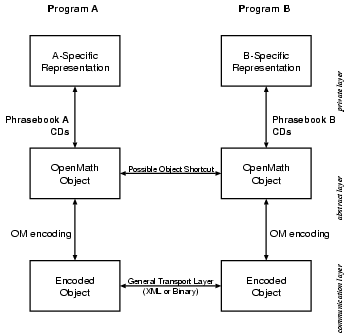
\includegraphics{om-arch}
  \caption{The \OM Architecture}\label{fig_om}
\end{figure}

The architecture of \OM is described in \ref{fig_om} and summarizes the interactions among
the different \OM components.  There are three layers of representation of a mathematical
object. The first is a private layer that is the internal representation used by an
application.  The second is an abstract layer that is the representation as an \OM object.
Note that these two layers may, in some cases, be the same.  The third is a communication
layer that translates the \OM object representation into a stream of bytes. An application
dependent program manipulates the mathematical objects using its internal representation,
it can convert them to \OM objects and communicate them by using the byte stream
representation of \OM objects.


\section{\OM Objects and Encodings}\label{sec_intro-obj}


\OM objects are representations of mathematical entities that
can be communicated among various software applications in a
meaningful way, that is, preserving their
\textquote{semantics}.

\OM objects and encodings are described in detail in \ref{cha_obj} and \ref{cha_enco}.



The standard endorses two encodings in \XML and binary
formats.
At the time of writing, these are the encodings
supported by most existing \OM tools and applications,
however they are not the only possible encodings of \OM
objects. Users who wish to define their own encoding
, are free to
do so provided that there is
a well-defined correspondence
between the new encoding and the abstract model defined in \ref{cha_obj}. 





\section{Content Dictionaries}\label{sec_intro-cd}


Content Dictionaries (CDs) are used to assign informal and formal
semantics to all symbols used in the \OM objects. They define the
symbols used to represent concepts arising in a particular area of
mathematics.


The Content Dictionaries are public, they represent the actual
common knowledge among \OM applications.  Content Dictionaries fix
the \textquote{meaning} of objects independently of the
application.  The application receiving the object may then recognize
whether or not, according to the semantics of the symbols defined in
the Content Dictionaries, the object can be transformed to the
corresponding internal representation used by the application.

\section{Additional Files}\label{sec_addnfiles} 
Several additional files are related to Content Dictionaries.  Signature Dictionaries
contain the signatures of symbols defined in some \OM Content Dictionary and their format
is endorsed by this standard.

Furthermore, the standard fixes how to define a specific set of Content Dictionaries as a
CDGroup.

Auxiliary files that define presentation and rendering or that are used for manipulating
and processing Content Dictionaries are not discussed by the standard.

\section{Phrasebooks}\label{sec_phrasebooks}

The conversion of an \OM object to/from the internal representation in a software
application is performed by an interface program called a \emph{Phrasebook}. The
translation is governed by the Content Dictionaries and the specifics of the
application. It is envisioned that a software application dealing with a specific area of
mathematics declares which Content Dictionaries it understands. As a consequence, it is
expected that the Phrasebook of the application is able to translate \OM objects built
using symbols from these Content Dictionaries to/from the internal mathematical objects of
the application.

\OM objects do not specify any computational behaviour, they merely represent mathematical
expressions.  Part of the \OM philosophy is to leave it to the application to decide what
it does with an object once it has received it.  \OM is not a query or programming
language. Because of this, \OM does not prescribe a way of forcing \textquote{evaluation}
or \textquote{simplification} of objects like $2+3$ or $\sin(x)$. Thus, the same object
$2+3$ could be transformed to $5$ by a computer algebra system, or displayed as $2+3$ by a
typesetting tool.

\chapter{\OM Objects}\label{cha_obj}

In this chapter we provide a self-contained description of \OM objects. We first do so by
means of an abstract grammar description (\ref{sec_omabs}) and then give a more informal
description (\ref{sec_omin}).

\section{Formal Definition of \OM Objects}\label{sec_omabs}


\OM represents mathematical objects as terms or as labelled
trees that are called \OM objects or \OM expressions. The definition
of an abstract \OM object is then the following.



\subsection{Basic \OM objects}\label{sec_basic} 

Basic \OM Objects form the leaves of the \OM Object tree.  A Basic \OM Object is of one of
the following.
 
\begin{itemize}
\item[(i)] Integer.  Integers in the mathematical sense, with no predefined range.  They
  are \textquote{infinite precision} integers (also called \textquote{bignums} in computer
  algebra).
\item[(ii)] \acronym{ieee} floating point number.  Double precision floating-point numbers
  following the \acronym{ieee} 754-1985 standard~\cite{ieee754_85}.
\item[(iii)] Character string.  A Unicode Character string. This also corresponds to
  \textquote{characters} in \XML.
\item[(iv)] Bytearray.  A sequence of bytes.
\item[(v)] Symbol.  A Symbol encodes three fields of information, a \emph{symbol name}, a
  \emph{Content Dictionary name}, and (optionally) a \emph{Content Dictionary base URI},
  The name of a symbol is a sequence of characters matching the regular expression
  described in \ref{sec_names}.  The Content Dictionary is the location of the definition
  of the symbol, consisting of a name (a sequence of characters matching the regular
  expression described in \ref{sec_names}) and, optionally, a unique prefix called a
  \emph{cdbase} which is used to disambiguate multiple Content Dictionaries of the same
  name.  There are other properties of the symbol that are not explicit in these fields
  but whose values may be obtained by inspecting the Content Dictionary specified. These
  include the symbol definition, formal properties and examples and, optionally, a
  \emph{Role} which is a restriction on where the symbol may appear in an \OM object.  The
  possible roles are described in \ref{sec_roles}.
\item[(vi)] Variable.  A Variable must have a \emph{name} which is a sequence of
  characters matching a regular expression, as described in \ref{sec_names}.
\end{itemize}


\subsection{Derived \OM Objects}\label{sec_derived}

Derived \OM objects are currently used as a way by which non-\OM
data is embedded inside an \OM object.
A derived \OM object is built as follows: 
\begin{itemize}
\item[(i)] If $A$ is \emph{not} an \OM object, then $\foreign{A}$ is an \OM
  \emph{foreign object}.  An \OM foreign object may optionally have an \emph{encoding}
  field which describes how its contents should be interpreted.
\end{itemize}




\subsection{\OM Objects}\label{sec_compound}
  
\OM objects are built recursively as follows.
\begin{itemize}
\item[(i)] Basic \OM objects are \OM objects.
(Note that derived \OM objects are
\emph{not} \OM objects, but are used to construct \OM
objects as described below.)
\item[(ii)] If $A_1$,\ldots, $A_n$ ($n>0$) are \OM objects, then
  \[\application{A_1,\ldots,A_n}\]
  is an \OM \emph{application object}.
\item[(iii)] If $S_1$,\ldots, $S_n$ are \OM objects, and $A$ is an \OM object, and If
  $A_1$,\ldots, $A_n$ ($n>0$) are \OM objects or \OM derived objects, then
  \[\attribution{A, A_1 S_1,\ldots,A_n S_n}\]
  is an \OM \emph{attribution object}. $A$ is the object \emph{stripped of attributions}.
  If $S_1$,\ldots, $S_n$ are referred to as \emph{keys} and $A_1$,\ldots, $A_n$ as their
  associated \emph{values}.  If, after recursively applying stripping to remove
  attributions, the resulting un-attributed object is a variable, the original attributed
  object is called an \emph{attributed variable}.

\item[(iv)] If $B$ and $C$ are \OM objects, and $v_1$,\ldots, $v_n$ ($n\geq 0$) are \OM variables or attributed
  variables, then
  \[\binding{B, v_1,\ldots,v_n, C}\]
  is an \OM \emph{binding object}.

\item[(v)]  If $S$ is an \OM symbol, and $A_1$,\ldots, $A_n$ ($n\geq 0$) are \OM objects or
\OM derived objects, then
  \[\error{S, A_1,\ldots,A_n}\]
  is an \OM \emph{error object}.
\end{itemize}
\OM objects that are contstructed via rules (ii) to (v) are jointly called \emph{compound
  \OM objects}
\subsection{\OM Symbol Roles}\label{sec_roles}


We say that an \OM symbol is used to \emph{construct}
an \OM object if it is the first child of an \OM application,
binding or error object, or an even-indexed child of an \OM
attribution object (i.e. the \emph{key} in a
\emph{(key, value)} pair).
The \emph{role} of an \OM symbol is a restriction
on how it may be used to construct a compound \OM object and, in the
case of the key in an attribution object, a clarification of how that
attribution should be interpreted.  The possible roles are:
\begin{enumerate}[(\em i\rm)]
\item \emph{binder} The symbol may appear as the first child of an \OM binding object.
\item \emph{attribution} The symbol may be used as key in an \OM attribution object,
  i.e. as the first element of a (key, value) pair, or in an equivalent context (for
  example to refer to the value of an attribution).  This form of attribution may be
  ignored by an application, so should be used for information which does not change the
  meaning of the attributed \OM object.
\item \emph{semantic-attribution} This is the same as \emph{attribution} except that it
  modifies the meaning of the attributed \OM object and thus cannot be ignored by an
  application, without changing the meaning.
\item \emph{error} The symbol may appear as the first child of an \OM error object.
\item \emph{application} The symbol may appear as the first child of an \OM application
  object.
\item \emph{constant} The symbol cannot be used to construct an \OM compound object.
\end{enumerate}
A symbol cannot have more than one role and cannot be used to construct a compound \OM
object in a way which requires a different role (using the definition of construct given
earlier in this section).  This means that one cannot use a symbol which binds some
variables to construct, say, an application object.  However it does not prevent the use
of that symbol as an \emph{argument} in an application object (where by argument we mean a
child with index greater than 1).
 
If no role is indicated then the symbol can be used anywhere.  Note that this is not the
same as saying that the symbol's role is \emph{constant}.

\section{Further Description of \OM Objects}\label{sec_omin}

Informally, an \OM \emph{object} can be
viewed as a tree and is also referred to as a term.  The objects at
the leaves of \OM trees are called \emph{basic
objects}.  The basic objects supported by \OM are:
\begin{description}
\item[Integer]  Arbitrary Precision
integers.
\item[Float] \OM floats are \acronym{ieee} 754 Double precision floating-point
  numbers. Other types of floating point number may be encoded in \OM by the use of
  suitable content dictionaries.
\item[Character strings]are sequences of characters. These characters come from the
  Unicode standard~\cite{UNICODE}.
\item[Bytearrays] are sequences of bytes. There is no \textquote{byte} in \OM as an object
  of its own. However, a single byte can of course be represented by a bytearray of length
  1.  The difference between strings and bytearrays is the following: a character string
  is a sequence of bytes with a fixed interpretation (as characters, Unicode texts may
  require several bytes to code one character), whereas a bytearray is an uninterpreted
  sequence of bytes with no intrinsic meaning.  Bytearrays could be used inside \OM errors
  to provide information to, for example, a debugger; they could also contain intermediate
  results of calculations, or \textquote{handles} into computations or databases.
\item[Symbols] are uniquely defined by the Content Dictionary in which they occur and by a
  name.  The form of these definitions is explained in \ref{cha_cd}.  Each symbol has no
  more than one definition in a Content Dictionary. Many Content Dictionaries may define
  differently a symbol with the same name (e.g. the symbol \lstinline|union| is defined
  as associative-commutative set theoretic union in a Content Dictionary \lstinline|set1|
  but another Content Dictionary, \lstinline|multiset1| might define a symbol
  \lstinline|union| as the union of multi-sets).
\item[Variables] are meant to denote parameters, variables or indeterminates (such as
  bound variables of function definitions, variables in summations and integrals,
  independent variables of derivatives).
\end{description} 
Derived \OM objects are constructed from non-\OM data.  They differ from bytearrays in
that they can have any structure.  Currently there is only one way of making a derived \OM
object.

\begin{description}
\item[Foreign] is used to import a non-\OM object into an \OM attribution.  Examples of
  its use could be to annotate a formula with a visual or aural rendering, an animation,
  etc.  They may also appear in \OM error objects, for example to allow an application to
  report an error in processing such an object.
\end{description}
The four following constructs can be used to make compound \OM objects out of basic or
derived \OM objects.

\begin{description}
\item[Application] constructs an \OM object from a sequence of one or more \OM
  objects. The first child of an application is referred to as its \textquote{head} while
  the remaining objects are called its \textquote{arguments}.  An \OM application object
  can be used to convey the mathematical notion of application of a function to a set of
  arguments.  For instance, suppose that the \OM symbol $\sin$ is defined in a suitable
  Content Dictionary, then $\application{\sin,x}$ is the abstract \OM object
  corresponding to $\sin(x)$.  More generally, an \OM application object can be used as a
  constructor to convey a mathematical object built from other objects such as a
  polynomial constructed from a set of monomials.  Constructors build inhabitants of some
  symbolic type, for instance the type of rational numbers or the type of polynomials.
  The rational number, usually denoted as $\frac12$, is
  represented by the \OM application object $\application{Rational,1,2}$. The symbol
  $Rational$ must be defined, by a Content Dictionary, as a
  constructor symbol for the rational numbers.

  \begin{figure}\centering
    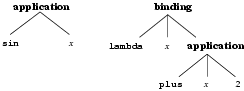
\includegraphics{lambda}
    \caption{The \OM application and binding objects for $\lambda x.x+2$ in tree-like notation.}\label{fig_obj}
  \end{figure}

\item[Binding] objects are
  constructed from an \OM object, and from a sequence of zero or more
  variables followed by another \OM object.  The first \OM object is
  the \textquote{binder} object. Arguments 2 to $n-1$ are always variables to
  be bound in the \textquote{body} which is the $n^{th}$ argument object. It
  is allowed to have no bound variables, but the binder object and the
  body should be present. Binding can be used to express functions or
  logical statements.  The function $\lambda x.x+2$, in which
  the variable $x$ is bound by $\lambda$, corresponds to a binding object having
  as binder the \OM symbol $lambda$: 
\[\binding{lambda,x,\application{plus,x,2}}\]

Phrasebooks are allowed to use $\alpha$-conversion in order to avoid clashes of
variable names. Suppose an object $\Omega$ contains an occurrence of the object
$\binding{B,v,C}$.  This object $\binding{B,v,C}$ can be replaced in $\Omega$ by
$\binding{B,z,C'}$ where $z$ is a variable not occurring free in $C$ and $C'$ is obtained
from $C$ by replacing each free (i.e., not bound by any intermediate $\mathbf{binding}$
construct) occurrence of $v$ by $z$.  This operation preserves the semantics of the object
$\Omega$. In the above example, a phrasebook is thus allowed to transform the object to,
e.g.
\[\binding{lambda,x,\application{plus,x,2}}\]


Repeated occurrences of the same variable in a binding operator
  are allowed. An \OM application should treat a binding with
  multiple occurrences of the same variable as equivalent to the
  binding in which all but the last occurrence of each variable is
  replaced by a new variable which does not occur free in the body of
  the binding.
  \[\binding{lambda,v,v,\application{times,v,v}}\]
is semantically
  equivalent to: 
  \[\binding{lambda,v',v,\application{times,v,v}}\]
  so that the resulting function is actually a constant in its first argument ($v'$ does
  not occur free in the body $\application{times,v,v}$.

\item[Attribution] decorates an object with a sequence of one or more pairs made up of an
  \OM symbol, the \textquote{attribute}, and an associated object, the \textquote{value of
    the attribute}.  The value of the attribute can be an \OM attribution object
  itself. As an example of this, consider the \OM objects representing groups,
  automorphism groups, and group dimensions. It is then possible to attribute an \OM
  object representing a group by its automorphism group, itself attributed by its
  dimension.

  \OM objects can be attributed with \OM foreign objects, which are containers for non-\OM
  structures.  For example a mathematical expression could be attributed with its spoken
  or visual rendering.



Composition of attributions, as in
\[\attribution{\attribution{A,S_1 A_1,\ldots, S_h A_h}, S_{h+1} A_{h+1},\ldots, S_n A_n}\] 
is semantically equivalent to a single attribution, that is
\[\attribution{A,S_1 A_1,\ldots, S_n A_n}\] 
The operation that produces an object with a single layer of attribution is called
\emph{flattening}.

Multiple attributes with the same name are allowed.  While the order of the given
attributes does not imply any notion of priority, potentially it could be significant. For
instance, consider the case in which $S_h=S_n$ ($h<n$) in the example above. Then, the
object is to be interpreted as if the value $A_n$ overwrites the value $A_h$.  (\OM
however does not mandate that an application preserves the attributes or their order.)


Attribution acts as either adornment annotation or as semantical annotation. When the key
has role \emph{attribution}, then replacement of the attributed object by the object
itself is not harmful and preserves the semantics. When the key has role
\emph{semantic-attribution} then the attributed object is modified by the attribution and
cannot be viewed as semantically equivalent to the stripped object. If the attribute lacks
the role specification then attribution is acting as adornment annotation.
  
Objects can be decorated in a multitude of ways.

An example of the use of an adornment attribution would be to indicate the colour in which
an \OM object should be displayed, for example $\attribution{A,colour,red}$.  Note that
both $A$ and $red$ are arbitary \OM objects whereas $color$ is a symbol.  An example of
the use of a semantic attribution would be to indicate the type of an object.  For example
the object $\attribution{A,type,t}$ represents the judgment stating that object $A$ has
type $t$. Note that both $A$ and $t$ are arbitary \OM objects whereas $type$ is a symbol.

\item[Error] is made up of an \OM symbol and a sequence of zero or more \OM objects. This
  object has no direct mathematical meaning.  Errors occur as the result of some treatment
  on an \OM object and are thus of real interest only when some sort of communication is
  taking place. Errors may occur inside other objects and also inside other errors.  Error
  objects might consist only of a symbol as in the object: $\error{S}$.
\end{description} 


\section{Names}\label{sec_names}

The names of symbols, variables and content dictionaries must conform to the production
\lstinline|Name| specified in the following grammar (which is identical to that for \XML
names in XML 1.1, \cite{xml_04}). Informally speaking, a name is a sequence of Unicode
\cite{UNICODE} characters which begins with a letter and cannot contain certain
punctuation and combining characters.  The notation \lstinline|#x...| represents the
hexadecimal value of the encoding of a Unicode character.  Some of the character values or
\emph{code points} in the following productions are currently unassigned, but this is
likely to change in the future as Unicode evolves \footnote{\label{xml1} We note that in
  XML 1 the name production explicitly listed the characters that were allowed, so all the
  characters added in versions of Unicode after 2.0 (which amounted to tens of thousands
  of characters) were not allowed in names.}


\begin{center}
\begin{tabular}{l@{$\longrightarrow$}p{10cm}}
Name & NameStartChar (NameChar)* \\
NameStartChar & 
\lstinline? ":" | [A-Z] | "_" | [a-z] | [#xC0-#xD6] | [#xD8-#xF6] |?\\
& \lstinline?[#xF8-#x2FF] | [#x370-#x37D] | [#x37F-#x1FFF] |?\\
& \lstinline?[#x200C-#x200D] | [#x2070-#x218F] | [#x2C00-#x2FEF] |?\\
& \lstinline?[#x3001-#xD7FF] | [#xF900-#xFDCF] | [#xFDF0-#xFFFD] |?\\
& \lstinline?[#x10000-#xEFFFF]? \\
NameChar & 
NameStartChar \lstinline?| "-" | "." | [0-9] | #xB7 | [#x0300-#x036F] |?\\
 & \lstinline?[#x203F-#x2040]? 
\end{tabular}
\end{center}

\paragraph{CD Base}

A cdbase must conform to the grammar for URIs described in
\cite{IETF2396}.  Note that if non-ASCII characters are
used in a CD or symbol name then when a URI for that symbol is
constructed it will be necessary to map the non-ASCII characters to a
sequence of octets.  The precise mechanism for doing this depends on
the URI scheme.


\paragraph{Note on content dictionary names}

It is a common convention to store a Content Dictionary in a file of
the same name, which can cause difficulties on many file systems.  If
this convention is to be followed then \OM
\emph{recommends} that the name be restricted to the
subset of the above grammar which is a legal POSIX
\cite{POSIX} filename, namely:

\begin{center}
\begin{tabular}{l@{$\longrightarrow$}p{10cm}}
Name & (PosixLetter \lstinline?| '_'?) (Char)*\\
Char &  PosixLetter \lstinline?| Digit | '.' | '-' | '_' ?\\
PosixLetter & \lstinline? 'a' | 'b' | ... | 'z' | 'A' | 'B' | ... | 'Z'?
\end{tabular}
\end{center}


\paragraph{Canonical URIs for Symbols}

To facilitate the use of \OM within a URI-based framework (such as RDF
\cite{rdf} or OWL \cite{owl}), we provide the
following scheme for constructing a canonical URI
for an \OM Symbol:
\begin{lstlisting}
URI = cdbase-value + '/' + cd-value + '#' + name-value
\end{lstlisting}
So for example the URI for the symbol with cdbase \url{http://www.openmath.org/cd}, cd
\lstinline|transc1| and name \lstinline|sin| is:
\begin{lstlisting}
http://www.openmath.org/cd/transc1#sin
\end{lstlisting}
In particular, this now allows us to refer uniquely to an \OM symbol from a
MathML document \cite{MathML_2003}:
\begin{lstlisting}
<mathml:csymbol xmlns:mathml="http://www.w3.org/1998/Math/MathML/"
                definitionURL="http://www.openmath.org/cd/transc1#sin">
  <mo> sin </mo> 
</csymbol>
\end{lstlisting}



\section{Summary}\label{sec_summary}

\begin{itemize}
\item \OM supports basic objects like integers, symbols, floating-point numbers, character
  strings, bytearrays, and variables.
\item \OM compound objects are of four kinds: applications, bindings, errors, and
  attributions.
\item \OM objects may be attributed with non-\OM objects via the use of foreign \OM
  objects.
\item \OM objects have the expressive power to cover all areas of computational
  mathematics.
\end{itemize}

Observe that an \OM application object is viewed as a \textquote{tree} by software
applications that do not understand Content Dictionaries, whereas a Phrasebook that
understands the semantics of the symbols, as defined in the Content Dictionaries, should
interpret the object as functional application, constructor, or binding accordingly. Thus,
for example, for some applications, the \OM object corresponding to $2+5$ may result in a
command that writes $7$.



\chapter{\OM Encodings}\label{cha_enco}


In this chapter, two encodings are defined that map between \OM
objects and byte streams.  These byte streams constitute a low level
representation that can be easily exchanged between processes (via
almost any communication method) or stored and retrieved from
files.




The first encoding is a character-based
encoding in \XML format.  In previous versions of the \OM Standard
this encoding was a restricted subset of the full legal \XML syntax.
In this version, however, we have removed all these restrictions so that
the earlier encoding is a strict subset of the existing one.  The
\XML encoding can be used, for example, to send \OM objects via
e-mail, cut-and-paste, etc. and to embed \OM objects in \XML
documents or to have \OM objects processed by \XML-aware
applications.


The second encoding is a binary encoding that is meant to be
used when the compactness of the encoding is important (inter-process
communications over a network is an example).


Note that these two encodings are sufficiently different for
auto-detection to be effective: an application reading the bytes can
very easily determine which encoding is used.


\section{The \XML Encoding}\label{sec_xml}

This encoding has been designed with two main goals in mind:
\begin{enumerate}
\item to provide an encoding that uses common character sets (so that it can easily be
  included in most documents and transport protocols) and that is both readable and
  writable by a human.
\item to provide an encoding that can be included (embedded) in \XML documents or
  processed by \XML-aware applications.
\end{enumerate}


\subsection{A Schema for the \XML Encoding}\label{ssec_xml}

The \XML encoding of an \OM object is defined by the Relax NG schema \cite{RELAX} given
below.  Relax NG has a number of advantages over the older XSD Schema format \cite{XSD},
in particular it allows for tighter control of attributes and has a modular, extensible
structure.  Although we have made the \XML form, which is given in \ref{app_openmath.rng},
normative, it is generated from the compact syntax given below.  It is also very easy to
restrict the schema to allow a limited set of \OM symbols as described in
\ref{app_relaxrestricted}.

Standard tools exist for generating a DTD or an XSD schema from a Relax NG Schema.
Examples of such documents are given in \ref{app_xsd}, respectively.

\lstinputlisting{openmath2.rnc}

\textbf{Note:} This schema specifies names as being of the \lstinline|xsd:NCName| type. At
the time of writing, W3C Schema types are defined in terms of XML 1 \cite{xml_98}.  This
limits the characters allowed in a name to a subset of the characters available in Unicode
2.0, which is far more restrictive than the definition for an \OM name given in
\ref{sec_names}.  It is expected that W3C Schema types will be augmented to match the new
XML 1.1 recommendation \cite{xml_04}, but for portability reasons applications should
avoid using the new XML 1.1 name characters unless they are absolutely required.  The XML
1.1 specification has a useful appendix giving advice on good strategies to use when
naming identifiers.

\subsection{Informal description of the \XML Encoding}\label{sec_xml-desc}

An encoded \OM object is placed inside an \lstinline|OMOBJ| element.  This 
element can contain the elements (and integers) described above.
 It can take an optional
\lstinline|version| (\XML) attribute which indicates to
which version of the \OM standard it conforms.  In previous versions of
this standard this attribute did not exist, so any \OM object without
such an attribute must conform to version 1 (or equivalently 1.1) of the
\OM standard.  Objects which conform to the description given in this
document should have \lstinline|version="2.0"|.



We briefly discuss the \XML encoding for each type of \OM object
starting from the basic objects.


\begin{description}
\item[Integers] are encoded using the
\lstinline|OMI| element around the sequence of their
digits in base 10 or 16 (most significant digit first).  White space
may be inserted between the characters of the integer representation,
this will be ignored.  After ignoring white space, integers written in
base 10 match the regular expression
\lstinline|-?[0-9]+|.  Integers written in base 16 match
\lstinline|-?x[0-9A-F]+|.  The integer 10 can be thus
encoded as \lstinline|<OMI> 10 </OMI> | or as
\lstinline|<OMI> xA </OMI> | but neither
\lstinline|<OMI> +10 </OMI>| nor
\lstinline|<OMI> +xA </OMI>| can be used.


The negative integer $-120$ can be encoded
as either as decimal \lstinline|<OMI> -120</OMI>| or as hexadecimal 
\lstinline|<OMI>-x78 </OMI>|.
\item[Symbols] are encoded using the \lstinline|OMS| element. This element has three
  (\XML) attributes \lstinline|cd|, \lstinline|name|, and \lstinline|cdbase|. The value
  of \lstinline|cd| is the name of the Content Dictionary in which the symbol is defined
  and the value of \lstinline|name| is the name of the symbol.  The optional
  \lstinline|cdbase| attribute is a URI that can be used to disambiguate between two
  content dictionaries with the same name.  If a symbol does not have an explicit
  \lstinline|cdbase| attribute, then it inherits its \lstinline|cdbase| from the first
  ancestor in the \XML tree with one, should such an element exist.  In this document we
  have tended to omit the \lstinline|cdbase| for clarity.
  
For example:
\begin{lstlisting}
<OMS cdbase="http://www.openmath.org/cd" cd="transc1" name="sin"/>
\end{lstlisting}
is the encoding of the symbol named \lstinline|sin| in the Content Dictionary named
\lstinline|transc1|, which is part of the collection maintained by the \OM Society.


As described in \ref{sec_names}, the three attributes of the \lstinline|OMS| can be used
to build a URI reference for the symbol, for use in contexts where URI-based referencing
mechanisms are used.  For example the URI for the above symbol is
\url{http://www.openmath.org/cd/transc1\#sin}.

Note that the role attribute described in \ref{sec_roles} is contained in the Content Dictionary and is not
part of the encoding of a symbol, also the \lstinline|cdbase| attribute need not
be explicit on each \lstinline|OMS| as it is inherited
from any ancestor element.
\item[Variables] are encoded using the \lstinline|OMV| element, with only one
  (\XML) attribute, \lstinline|name|, whose value is the variable name. For instance, the
  encoding of the object representing the variable $x$ is: \lstinline|<OMV name="x"/>|
\item[Floating-point numbers] are encoded using the \lstinline|OMF| element
  that has either the (\XML) attribute \lstinline|dec| or the (\XML) attribute
  \lstinline|hex|. The two (\XML) attributes cannot be present simultaneously. The value
  of \lstinline|dec| is the floating-point number expressed in base 10, using the common
  syntax:

\begin{lstinline}
(-?)([0-9]+)?("."[0-9]+)?([eE](-?)[0-9]+)?
\end{lstinline}

or one of the special values: INF, -INF or NaN.

The value of \lstinline|hex| is a base 16 representation of the 64 bits of the
\acronym{ieee} Double.  Thus the number represents mantissa, exponent, and sign from
lowest to highest bits using a least significant byte ordering.  This consists of a string
of 16 digits \lstinline|0|-\lstinline|9|, \lstinline|A|-\lstinline|F|.
  

For example, both \lstinline|<OMF dec="1.0e-10"/>| and 
   \lstinline|<OMF hex="3DDB7CDFD9D7BDBB"/>|
  are valid representations of the floating point number $1\times 10^{-10}$.

 
  The symbols \lstinline|INF|, \lstinline|-INF| and \lstinline|NaN| represent positive
  and negative infinity, and \emph{not a number} as defined in \cite{ieee754_85}.  Note
  that while infinities have a unique representation, it is possible for NaNs to contain
  extra information about how they were generated and if this informations is to be
  preserved then the hexadecimal representation must be used.  For example
  \lstinline|<OMF hex="FFF8000000000000"/>| and 
\lstinline|<OMFhex="FFF8000000000001"/>| are both hexadecimal representations of NaNs.
\item[Character strings] are encoded using the \lstinline|OMSTR| element.  Its
  content is a Unicode text. Note that as always in \XML the characters \lstinline|<| and
  \lstinline|\&| need to be represented by the entity references \lstinline|\&lt;|
  and \lstinline|\&amp;| respectively.
\item[Bytearrays] are encoded using the \lstinline|OMB| element. Its content is
  a sequence of characters that is a base64 encoding of the data.  The base64 encoding is
  defined in \acronym{rfc} 2045 \cite{rfc2045}.  Basically, it represents an arbitrary
  sequence of octets using 64 \textquote{digits} (\lstinline|A| through \lstinline|Z|,
  \lstinline|a| through \lstinline|z|, \lstinline|0| through \lstinline|9|,
  \lstinline|+| and /, in order of increasing value). Three octets are represented as
  four digits (the \lstinline|=| character is used for padding at the end of the
  data). All line breaks and carriage return, space, form feed and horizontal tabulation
  characters are ignored. The reader is referred to \cite{rfc2045} for more detailed
  information.
\end{description}
 
\begin{description}
\item[Applications] are encoded using the \lstinline|OMA| element. The
  application whose head is the \OM object $e_0$ and whose arguments
  are the \OM objects $e_1$, \ldots, $e_n$ is encoded as \lstinline|<OMA>|
  $C_0$ $C_1$\ldots $C_n$ \lstinline|</OMA>| where $C_i$ is the encoding of
  $e_i$.


For example, $\application{sin,x}$ is encoded as:
\begin{lstlisting}
<OMA>  
  <OMS cd="transc1" name="sin"/> 
  <OMV name="x"/>  
</OMA>
\end{lstlisting}
  provided that the symbol \lstinline|sin| is defined to be a function
  symbol in a Content Dictionary named \lstinline|transc1|.
\item[Binding] is encoded using the \lstinline|OMBIND| element.  The binding by the \OM
  object $b$ of the \OM variables $x_1$, $x_2$,\ldots, $x_n$ in the object $c$ is encoded
  as \lstinline|<OMBIND>| $B$ \lstinline|<OMBVAR>| $X_1$,\ldots, $X_n$
  \lstinline|</OMBVAR>| $C$ \lstinline|</OMBIND>| where $B$, $C$, and $X_i$ are the
  encodings of $b$, $c$ and $x_i$, respectively.

  For instance the encoding of $\binding{\lambda,x,\application{\sin,x}}$is:
\begin{lstlisting}
<OMBIND>
  <OMS cd="fns1" name="lambda"/>  
  <OMBVAR><OMV name="x"/></OMBVAR>  
  <OMA>
    <OMS cd="transc1" name="sin"/> 
    <OMV name="x"/>  
  </OMA>
</OMBIND>
\end{lstlisting}
  
Binders are defined in  Content Dictionaries, in particular,
  the symbol \lstinline|lambda| is defined in the Content Dictionary
  \lstinline|fns1| for functions over functions.
\item[Attributions] are encoded using the \lstinline|OMATTR| element.  If
  the \OM object $e$ is attributed with ($s_1$, $e_1$), \ldots, 
  ($s_n$, $e_n$) pairs (where $s_i$ are the attributes), it is encoded
  as \lstinline|<OMATTR>| \lstinline|<OMATP>| $S_1$ $C_1$ \ldots $S_n$ $C_n$ \lstinline|</OMATP>| $E$ \lstinline|</OMATTR>| where $S_i$ is the encoding of the
  symbol $s_i$, $C_i$ of the object $e_i$ and $E$ is the encoding of
  $e$.


Examples are the use of attribution to decorate a group by its
  automorphism group:
\begin{lstlisting}
<OMATTR>    
  <OMATP>
    <OMS cd="groups" name="automorphism_group" />  
    [..group-encoding..] 
  </OMATP>  
  [..group-encoding..] 
</OMATTR>
\end{lstlisting}
or to express the type of a variable:
\begin{lstlisting}
<OMATTR>    
  <OMATP>
    <OMS cd="ecc" name="type" /> 
    <OMS cd="ecc" name="real" />
  </OMATP> 
  <OMV name="x" />
</OMATTR>
\end{lstlisting}

A special use of attributions is to associate non-\OM data with an \OM object.  This is
done using the \lstinline|OMFOREIGN| element.  The children of this element must be
well-formed \XML.  For example the attribution of the \OM object $\sin(x)$ with its
representation in Presentation MathML is:
\begin{lstlisting}
<OMATTR>
  <OMATP>
    <OMS cd="annotations1" name="presentation-form"/>  
    <OMFOREIGN encoding="MathML-Presentation">
      <math xmlns="http://www.w3.org/1998/Math/MathML">
        <mi>sin</mi><mfenced><mi>x</mi></mfenced>
      </math>
    </OMFOREIGN>  
  </OMATP>
  <OMA>
   <OMS cd="transc1" name="sin"/> 
   <OMV name="x"/>  
  </OMA>
</OMATTR>
\end{lstlisting}
Of course not everything has a natural XML encoding in this way and
often the contents of a \lstinline|OMFOREIGN| will just
be data or some kind of encoded string.  For example the attribution
of the previous object with its LaTeX representation could be achieved
as follows:
\begin{lstlisting}
<OMATTR>
  <OMATP>
    <OMS cd="annotations1" name="presentation-form"/>  
    <OMFOREIGN encoding="text/x-latex">\sin(x)</OMFOREIGN>  
  </OMATP>
  <OMA>
    <OMS cd="transc1" name="sin"/> 
    <OMV name="x"/>  
  </OMA>
</OMATTR>
\end{lstlisting}
For a discussion on the use of the \lstinline|encoding|
attribute see \ref{sec_compl_omforeign}.
\item[Errors] are encoded using the \lstinline|OME| element. The error whose symbol is $s$
  and whose arguments are the \OM objects or \OM derived objects $e_1$, \ldots, $e_n$ is
  encoded as \lstinline|<OME>| $C_s$ $C_1$\ldots $C_n$ \lstinline|</OME>| where $C_s$ is
  the encoding of $s$ and $C_i$ the encoding of $e_i$.

  If an \lstinline|aritherror| Content Dictionary contained a \lstinline|DivisionByZero|
  symbol, then the object
  $\error{DivisionByZero{\application{divide,x,0}}}$ would be encoded as follows:

\begin{lstlisting}
<OME>
  <OMS cd="aritherror" name="DivisionByZero"/>  
  <OMA>
    <OMS cd="arith1" name="divide" />
    <OMV name="x"/>  
    <OMI> 0 </OMI>
  </OMA> 
 </OME>
\end{lstlisting}

  

If a \lstinline|mathml| Content Dictionary contained an
  \lstinline|unhandled_csymbol| symbol, then an \OM to
MathML translator might return an error such as:
\begin{lstlisting}
<OME>
  <OMS cd="mathml" name="unhandled_csymbol"/>  
  <OMFOREIGN encoding="MathML-Content">
    <mathml:csymbol xmlns:mathml="http://www.w3.org/1998/Math/MathML/"
                    definitionURL="http://www.nag.co.uk/Airy#A">
      <mathml:mo>Ai</mathml:mo>
    </mathml:csymbol>
  </OMFOREIGN> 
 </OME>
\end{lstlisting}


 Note that it is possible to embed fragments
of valid \OM inside an \lstinline|OMFOREIGN| element but that it
cannot contain invalid \OM.  In addition, the arguments to an
\lstinline|OMERROR| must be well-formed \XML.  If an
application wishes to signal that the \OM it has received is invalid or
is not well-formed then the offending data must be encoded as a string.
For example:
\begin{lstlisting}
<OME>
  <OMS cd="parser" name="invalid_XML"/>  
  <OMSTR>
    &ltOMA> <OMS name="cos" cd="transc1">
      <OMV name="v"> </OMA>
  </OMSTR> 
 </OME>
\end{lstlisting}
Note that the \textquote{<} and \textquote{>} characters have been escaped as is usual in
an \XML document.
\item[References] \OM integers, floating point numbers, character strings, bytearrays,
  applications, binding, attributions can also be encoded as an empty \lstinline|OMR|
  element with an \lstinline|href| attribute whose value is the value of a URI referencing
  an id attribute of an \OM object of that type.  The \OM element represented by this
  \lstinline|OMR| reference is a copy of the \OM element referenced \lstinline|href|
  attribute. Note that this copy is \emph{structurally equal}, but not identical to the
  element referenced. These URI refererences will often be relative, in which case they
  are resolved using the base URI of the document containing the \OM.

 For instance, the \OM object

\begin{lstlisting}
 <math id="nestedap" display="block">
   <mrow>
     <mi mathvariant="bold">application</mi>
     <mrow>
       <mo fence="true">(</mo>
       <mrow>
         <mi>f</mi>
         <mo separator="true">,</mo>
         <mi mathvariant="bold">application</mi>
         <mrow>
           <mo fence="true">(</mo>
           <mrow>
             <mi>f</mi>
             <mo separator="true">,</mo>
             <mi mathvariant="bold">application</mi>
             <mrow>
               <mo fence="true">(</mo>
               <mrow><mi>f</mi><mo separator="true">,</mo><mi>a</mi><mo separator="true">,</mo><mi>a</mi></mrow>
               <mo fence="true">)</mo>
             </mrow>
             <mo separator="true">,</mo>
             <mi mathvariant="bold">application</mi>
             <mrow>
               <mo fence="true">(</mo>
               <mrow><mi>f</mi><mo separator="true">,</mo><mi>a</mi><mo separator="true">,</mo><mi>a</mi></mrow>
               <mo fence="true">)</mo>
             </mrow>
             <mo fence="true">)</mo>
           </mrow>
           <mo separator="true">,</mo>
           <mi mathvariant="bold">application</mi>
           <mrow>
             <mo fence="true">(</mo>
             <mrow>
               <mi>f</mi>
               <mo separator="true">,</mo>
               <mi mathvariant="bold">application</mi>
               <mrow>
                 <mo fence="true">(</mo>
                 <mrow><mi>f</mi><mo separator="true">,</mo><mi>a</mi><mo separator="true">,</mo><mi>a</mi></mrow>
                 <mo fence="true">)</mo>
               </mrow>
               <mo separator="true">,</mo>
               <mi mathvariant="bold">application</mi>
               <mrow>
                 <mo fence="true">(</mo>
                 <mrow><mi>f</mi><mo separator="true">,</mo><mi>a</mi><mo separator="true">,</mo><mi>a</mi></mrow>
                 <mo fence="true">)</mo>
               </mrow>
               <mo fence="true">)</mo>
             </mrow>
           </mrow>
           <mo fence="true">)</mo>
         </mrow>
       </mrow>
     </mrow>
   </mrow>
 </math>
\end{lstlisting}
can be encoded in the \XML encoding as either one of the \XML encodings given in
\ref{fig_shared_vs_unshared} (and some intermediate versions as well).
\end{description}

\begin{figure}\centering
\caption{Shared vs. unshared representations}\label{fig_shared_vs_unshared}
    
\begin{lstlisting}
<OMOBJ version="2.0">         <OMOBJ version="2.0">
  <OMA>                         <OMA>
    <OMV name="f"/>               <OMV name="f"/> 
    <OMA>                         <OMA id="t1">
      <OMV name="f"/>               <OMV name="f"/>
      <OMA>                         <OMA id="t11">
        <OMV name="f"/>               <OMV name="f"/>
        <OMV name="a"/>               <OMV name="a"/>
        <OMV name="a"/>               <OMV name="a"/>
      </OMA>                        </OMA>
      <OMA>                         <OMR href="#t11"/>
        <OMV name="f"/>
        <OMV name="a"/> 
        <OMV name="a"/>
      </OMA>                                
    </OMA>                      </OMA>
    <OMA>                       <OMR href="#t1"/>
      <OMV name="f"/>
      <OMA>
        <OMV name="f"/>
        <OMV name="a"/>
        <OMV name="a"/>
      </OMA>
      <OMA>
        <OMV name="f"/>
        <OMV name="a"/>
        <OMV name="a"/>
      </OMA>
    </OMA>
  </OMA>
</OMOBJ>                     </OMOBJ>
\end{lstlisting}
\end{figure}


\subsection{Some Notes on References}\label{sec_references}

We say that an \OM element dominates all its children and all elements
they dominate. An \lstinline|OMR| element dominates its target,
i.e. the element that carries the \lstinline|id| attribute pointed to
by the \lstinline|xref| attribute. For instance in the representation
in \ref{fig_shared_vs_unshared}, the
\lstinline|OMA| element with \lstinline|id="t1"| and
also the second \lstinline|OMR| dominate the
\lstinline|OMA| element with \lstinline|id="t11"|.



\subsubsection{An Acyclicity Constraint}\label{sec_acyclicity}

The occurrences of the \lstinline|OMR| element must obey the following global
\emph{acyclicity constraint}: An \OM element may not dominate itself.


Consider for instance the following (illegal) \XML representation
\begin{lstlisting}
<OMOBJ version="2.0">
  <OMA id="foo">
    <OMS cd="arith1" name="divide"/>
    <OMI>1</OMI>
    <OMA>
       <OMS cd="arith1" name="plus"/>
       <OMI>1</OMI>
       <OMR xref="foo"/>
    </OMA> 
  </OMA>
</OMOBJ>
\end{lstlisting}

Here, the \lstinline|OMA| element with
\lstinline|id="foo"| dominates its third child, which dominates the
\lstinline|OMR| element, which dominates its target: the element with
\lstinline|id="foo"|. So by transitivity, this element dominates itself, and
by the acyclicity constraint, it is not the \XML representation of an \OM
element. Even though it could be given the interpretation of the continued fraction
<math display="block">
 <mfrac>
   <mn>1</mn>
   <mrow>
     <mn>1</mn>
     <mo>+</mo>
     <mfrac>
       <mn>1</mn>
       <mrow>
         <mn>1</mn>
         <mo>+</mo>
         <mfrac><mn>1</mn><mi>...</mi></mfrac>
       </mrow>
     </mfrac>
   </mrow>
 </mfrac>
</math> this would correspond to an infinite tree of applications,
which is not admitted by the structure of \OM objects described
in \ref{cha_obj}.


Note that the acyclicity constraints is not restricted
to such simple cases, as the example in \ref{fig_sharing_between}
shows.


\begin{figure}\centering
\caption{Sharing between \OM objects (A cycle of order 2).}\label{fig_sharing_between}
\begin{lstlisting}
<OMOBJ version="2.0">                   <OMOBJ version="2.0">
  <OMA id="bar">                         <OMA id="baz">
    <OMS cd="arith1" name="plus"/>         <OMS cd="arith1" name="plus"/>
    <OMI>1</OMI>                           <OMI>1</OMI>
    <OMR xref="baz"/>                      <OMR xref="bar"/>
  </OMA>                                 </OMA>
</OMOBJ>                               </OMOBJ>
\end{lstlisting}
\end{figure}

 Here, the \lstinline|OMA| with
\lstinline|id="bar"| dominates its third child, the
\lstinline|OMR| with \lstinline|xref="baz"|,
which dominates its target \lstinline|OMA| with
\lstinline|id="baz"|, which in turn dominates its third
child, the \lstinline|OMR| with
\lstinline|xref="bar"|, this finally dominates its
target, the original \lstinline|OMA| element with
\lstinline|id="bar"|. So this pair of \OM objects
violates the acyclicity constraint and is not the \XML
representation of an \OM object.




\subsubsection{Sharing and Bound Variables}\label{sec_sharing_bvars}

Note that the \lstinline|OMR| element is a \emph{syntactic} referencing mechanism: an
\lstinline|OMR| element stands for the exact \XML element it points to. In particular,
referencing does not interact with binding in a semantically intuitive way, since it
allows for variable capture. Consider for instance the following \XML representation:
\begin{lstlisting}
<OMBIND id="outer">
  <OMS cd="fns1" name="lambda"/>
  <OMBVAR><OMV name="X"/></OMBVAR>
  <OMA>
    <OMV name="f"/>
    <OMBIND id="inner">
      <OMS cd="fns1" name="lambda"/>
      <OMBVAR><OMV name="X"/></OMBVAR>
      <OMR id="copy" href="#orig"/>
    </OMBIND>
    <OMA id="orig"><OMV name="g"/><OMV name="X"/></OMA>
  </OMA>
</OMBIND>
\end{lstlisting}
it represents the \OM object
\[\binding{\lambda,X,\application{f,\binding{\lambda,X,\application{g,X},\application{g,X}}}}\]
which has two sub-terms of the form $\application{g,X}$, one with \lstinline|id="orig"|
(the one explicitly represented) and one with \lstinline|id="copy"|, represented by the
\lstinline|OMR| element. In the original, the variable $X$ is bound by the \emph{outer}
\lstinline|OMBIND| element, and in the copy, the variable $X$is bound by the \emph{inner}
\lstinline|OMBIND| element. We say that the inner \lstinline|OMBIND| has captured the
variable $X$.

It is well-known that variable capture does not conserve semantics. For instance, we could
use $\alpha$-conversion to rename the inner occurrence of $X$ into, say, $Y$ arriving at
the (same) object
\[\binding{\lambda,X,\application{f,\binding{\lambda,Y,\application{g,Y},\application{g,X}}}}\]
Using references that capture variables in this way can easily lead to representation
errors, and is not recommended.

\subsection{Embedding \OM in \XML Documents}\label{xmldoc}
     
The above encoding of \XML encoded \OM specifies the grammar to be used in files that
encode a single \OM object, and specifies the character streams that a conforming \OM
application should be able to accept or produce.


When embedding \XML encoded \OM objects into a larger \XML document one may wish, or need,
to use other \XML features. For example use of extra \XML attributes to specify \XML
Namespaces~\cite{xmlns} or \lstinline|xml:lang| attributes to specify the language used
in strings~\cite{xml_04}.

If such \XML features are used then the \XML application controlling the document must, if
passing the \OM fragment to an \OM application, remove any such extra attributes and must
ensure that the fragment is encoded according to the schema specified above.

\section{The Binary Encoding}\label{sec_binary}

The binary encoding was essentially designed to be more compact than the \XML encodings,
so that it can be more efficient if large amounts of data are involved. For the current
encoding, we tried to keep the right balance between compactness, speed of encoding and
decoding and simplicity (to allow a simple specification and easy implementations).

\subsection{A Grammar for the Binary Encoding}\label{sec_binary_grammar}

\def\abyte{[\_]}\def\fourbytes{\ensuremath{\{\_\}}}
\begin{figure}\centering\footnotesize
\begin{center}
\begin{tabular}{lcp{6cm}lcp{5cm}}
  start  &  $\longrightarrow$& [24] object [25] 
           &  $|$ &  [24+64] [$m$]  [$n$] object [25]\\
   object  & $\longrightarrow$& basic
      & $|$ &  compound &\\
      & $|$ & cdbase
      & $|$ & foreign \\
      & $|$ & reference &\\
    basic & $\longrightarrow$ &  integer  
      & $|$ &  float \\
      & $|$ &  variable 
      & $|$ &  symbol   \\
      & $|$ &  string 
      & $|$ &  bytearray \\
    integer  & $\longrightarrow$&[1] \abyte 
      & $|$ & [1+64] [$n$] id:$n$ \abyte\\
      & $|$ &  [1+32] \abyte  & &  \\
      & $|$ &  [1+128] \fourbytes 
      &  $|$ & [1+64+128] {$n$} id:$n$ \fourbytes\\
      & $|$ &  [1+32+128] \fourbytes  &
      &  &\\
      & $|$ &  [2] [$n$] \abyte digits:$n$
      & $|$ & [2+64] [$n$] [$m$] \abyte digits:$n$ id:$m$\\
      & $|$ & [2+32] [$n$] \abyte digits:$n$ & 
      &  \\
      & $|$ & [2+128] {$n$} \abyte digits:$n$
      & $|$ & [2+64+128] {$n$} {$n$} \abyte digits:$n$ id:$n$\\
      & $|$ & [2+32+128] {$n$} \abyte digits:$n$
      & & \\
   float  & $\longrightarrow$& [3] \fourbytes\fourbytes 
       & $|$ & [3+64] [$n$] id:$n$ \fourbytes\fourbytes\\
       & &
       & $|$ & [3+64+128] {$n$} id:$n$ \fourbytes\fourbytes\\
    variable  & $\longrightarrow$& [5] [$n$] varname:$n$
       & $|$ & [5+64] [$n$] [$m$] varname:$n$ id:$m$\\
       & $|$ & [5+128] {$n$} varname:$n$
       & $|$ & [5+64+128] {$n$} {$m$} varname:$n$ id:$m$\\
    symbol & $\longrightarrow$& [8] [$n$] [$m$] cdname:$n$ symbname:$m$
       & $|$ & [8+64] [$n$] [$m$] [$k$] cdname:$n$ symbname:$m$ id:$k$\\
       & $|$ & [8+128] {$n$} {$m$} cdname:$n$ symbname:$m$
       & $|$ & [8+64+128] {$n$} {$m$} {$k$} cdname:$n$ symbname:$m$ id:$k$\\
    string  & $\longrightarrow$& [6] [$n$] bytes:$n$
       & $|$ & [6+64] [$n$] bytes:$n$\\
       & $|$ & [6+32] [$n$] bytes:$n$ & & \\
       & $|$ & [6+128] {$n$} bytes:$n$
       & $|$ & [6+64+128] {$n$} {$m$} bytes:$n$ id:$m$\\
       & $|$ & [6+32+128] {$n$} bytes:$n$
       & & \\
       & $|$ & [7] [$n$] bytes:$2n$ 
       & $|$ & [7+64] [$n$] [$m$]bytes:$n$id:$m$ \\
       & $|$ & [7+32] [$n$] bytes:$2n$
       & & \\
       & $|$ & [7+128] {$n$} bytes:$2n$
       & $|$ & [7+64+128] {$n$} {$m$} bytes:$2n$ id:$m$\\
       & $|$ & [7+32+128] {$n$} bytes:$2n$ &&\\
   bytearray  & $\longrightarrow$& [4] [$n$] bytes:$n$
       & $|$ & [4+64] [$n$] [$m$] bytes:$n$ id:$m$\\
       & $|$ & [4+32] [$n$] bytes:$n$ && \\
       & $|$ & [4+128] {$n$} bytes:$n$
       & $|$ & [4+64+128] {$n$} {$m$} bytes:$n$ id:$m$\\
       & $|$ & [4+32+128] {$n$} bytes:$n$ && \\
    cdbase & $\longrightarrow$& [9] [$n$] uri:$n$ 
       &&\\
       & $|$ & [9+128] {$n$} uri:$n$ && \\
    foreign &$\longrightarrow$& [12] [$n$] [$m$] bytes:$n$ bytes:$m$
       & $|$ & [12+64] [$n$] [$m$] [$k$] bytes:$n$ bytes:$m$ id:$k$ \\
       & $|$ & [12+32] [$n$] [$m$] bytes:$n$ bytes:$m$ 
       &    & \\
       & $|$ & [12+128] {$n$} {$m$} bytes:$n$ bytes:$m$
       & $|$ & [12+64+128] {$n$} {$m$} {$k$} bytes:$n$ bytes:$m$ id:$k$\\
       & $|$ & [12+32+128] {$n$} {$m$} bytes:$n$ bytes:$m$
       &    &\\
   compound & $\longrightarrow$& application
      & $|$ & binding \\
      & $|$ & attribution
      & $|$ & error \\
   application & $\longrightarrow$ & [16] object objects [17] 
       & $|$ & [16+64] [$m$] id:$m$ object objects [17]\\
       &&
       & $|$ & [16+64+128] {$m$} id:$m$ object objects [17]\\
    binding & $\longrightarrow$&[26] object bvars object [27] 
       & $|$ & [26+64] [$m$] id:$m$ object bvars object [27] \\
       & & 
       & $|$ & [26+64+128] {$m$} id:$m$ object bvars object [27]\\
    attribution & $\longrightarrow$&[18] attrpairs object [19] 
       & $|$ & [18+64] [$m$] id:$m$ attrpairs object [19]\\
       & & 
       & $|$ & [18+64+128] {$m$} id:$m$ attrpairs object [19]\\
     error &  $\longrightarrow$&[22] symbol objects [23] 
        & $|$ & [22+64] [$m$] id:$m$ symbol objects [23]\\
       & & 
      & $|$ & [22+64+128] {$m$} id:$m$ symbol objects [23]\\
     attrpairs  & $\longrightarrow$&[20] pairs [21] 
        & $|$ & [20+64] [$m$] id:$m$ pairs [21]\\
       & & 
      & $|$ & [20+64+128] {$m$} id:$m$ pairs [21]\\
    pairs  & $\longrightarrow$&symbol object &\\
      & $|$ & symbol object pairs &\\
    bvars  & $\longrightarrow$&[28] vars [29] 
      & $|$ & [28+64] [$m$] id:$m$ vars [29]\\
      & & 
      & $|$ & [28+64+128] {$m$} id:$m$ vars [29]\\
   vars  & $\longrightarrow$& \emph{empty}
      & $|$ & attrvar vars &\\
   attrvar  & $\longrightarrow$&variable &\\
      & $|$ & [18] attrpairs attrvar [19] 
      & $|$ & [18+64] [$m$] id:$m$ attrpairs attrvar [19]\\
      & & 
      & $|$ & [18+64+128] {$m$} id:$m$ attrpairs attrvar [19]\\
  objects  & $\longrightarrow$&\emph{empty} 
      & $|$ & object objects \\
  reference &$\longrightarrow$& internal\_reference
      & $|$ & external\_reference \\
  internal\_reference  & $\longrightarrow$&[30] \abyte
      & $|$ & [30+128] \fourbytes \\
  external\_reference  & $\longrightarrow$& [31] [$n$] uri:$n$
      & $|$ & [31+128] {$n$} uri:$n$
\end{tabular}
\end{center}
\caption{Grammar of the binary encoding of \OM objects.}\label{fig_bin-enc}
\end{figure}
  
\ref{fig_bin-enc} gives a grammar for the binary encoding (\textquote{start} is the start
symbol).

The following conventions are used in this section: [$n$] denotes a byte whose value is
the integer $n$ ($n$ can range from 0 to 255), {$m$} denotes four bytes representing the
(unsigned) integer $m$ in network byte order, \abyte denotes an arbitrary byte, \fourbytes denotes
an arbitrary sequence of four bytes.  Finally, \emph{empty} stands for the empty list of
tokens.

\emph{xxxx}:$n$, where \emph{xxxx} is one of \emph{symbname}, \emph{cdname},
\emph{varname}, \emph{uri}, \emph{id}, \emph{digits}, or \emph{bytes} denotes a sequence
of $n$ bytes that conforms to the constraints on \emph{xxxx} strings. For instance, for
\emph{symbname}, \emph{varname}, or \emph{cdname} this is the regular expression described
in \ref{sec_names}, for \emph{uri} it is the grammar for URIs in \cite{IETF2396}.

\subsection{Description of the Grammar}\label{sec_bin-desc}
  
An \OM object is encoded as a sequence of bytes starting with the begin object tag (values
24 and 88) and ending with the end object tag (value~25). These are similar to the
\lstinline|<OMOBJ>| and \lstinline|</OMOBJ>| tags of the \XML encoding. Objects with
start token [88] have two additional bytes $m$ and $n$ that characterize the version
($m.n$) of the encoding directly after the start token. This is similar to
\lstinline|<OMOBJ version="m.n">|.

The encoding of each kind of \OM object begins with a tag that is a single byte, holding a
\emph{token identifier} that describes the kind of object, two flags, and a status
bit. The identifier is stored in the first five bits (1 to 5). Bit 6 is used as a
\emph{status bit} which is currently only used for managing streaming of some basic
objects. Bits 7 and 8 are the \emph{sharing flag} and the \emph{long flag}. The sharing
flag indicates that the encoded object may be shared in another (part of an) object
somewhere else (see \ref{sec_sharing_references}). Note that if the sharing flag is set
(in the right column of the grammar in \ref{fig_bin-enc}, then the encoding includes a
representation of an identifier that serves as the target of a reference (internal with
token identifier 30 or external with token identifier 31). If the long flag is set, this
signifies that the names, strings, and data fields in the encoded \OM object are longer
than 255 bytes or characters.

The concept of structure sharing in \OM encodings and in particular the sharing bit in the
binary encoding has been introduced in \OM~2 (see section \ref{sec_sharing_references} for
details). The binary encoding in \OM~2 leaves the tokens with sharing flag 0 unchanged to
ensure \OM~1 compatibility. To make use of functionality like the version attribute on the
\OM object introduced in \OM~2, the tokens with sharing flag 1 should be used.


To facilitate the streaming of \OM objects, some basic objects (integers, strings,
bytearrays, and foreign objects) have variant token identifiers with the fifth bit
set. The idea behind this is that these basic objects can be split into packets. If the
fifth bit is not set, this packet is the final packet of the basic object. If the bit is
set, then more packets of the basic object will follow directly after this one. Note that
all packets making up a basic object must have the same token identifier (up to the fifth
bit). In \ref{fig_bin-enc_stream} we have represented an integer that is split up into
three packets.

Here is a description of the binary encodings of every kind of \OM object:

\begin{description}
\item[Integers] are encoded depending on how large they
      are. There are four possible formats.  Integers between -128 and 127 are
      encoded as the small integer tags (token
	identifier 1) followed by a single byte that is the 
      value of the integer (interpreted as a signed character). For
      example 16 is encoded as \lstinline|0x01 0x10|.  Integers between
      $-2^{31}$  (-2147483648) and $2^{31-1}$  (2147483647) are encoded as
      the small integer tag with the long flag set followed by the integer
      encoded in little endian format in four bytes (network byte order:
      the most significant byte comes first). For example, 128 is encoded
      as \lstinline|0x81| \lstinline|0x00000080|.  The most
      general encoding begins 
      with the big integer tag (token identifier 2) with the long flag set
      if the number of bytes in the encoding of the digits is greater or
      equal than 256. It is followed by the length (in bytes) of the
      sequence of digits, encoded on one byte (0 to 255, if the long flag
      was not set) or four bytes (network byte order, if the long flag was
      set).  It is then followed by a byte describing the sign and the
      base.  This 'sign/base' byte is \lstinline|+|
      (\lstinline|0x2B|) or \lstinline|-|
      (\lstinline|0x2D|) for the sign or-ed with the base mask bits
      that can be \lstinline|0| for base 10 
      or \lstinline|0x40| for base 16 or
	\lstinline|0x80| for \textquote{base 256}.  It is
      followed by the 
      sequence of digits (as 
      characters for bases 10 and 16 as in the \XML
	encoing, and as bytes for base 256) in their natural
      order.  For example, the decimal
	number 8589934592
      ($2^{33}$) is encoded  as
\begin{lstlisting}
0x02 0x0A 0x2B 0x38 0x35 0x38 0x39 0x39 0x33 0x34 0x35 0x39 0x32
\end{lstlisting}
      and the
      hexadecimal number
      \lstinline|xffffff1| is 
      encoded as 
\begin{lstlisting}
  0x02 0x08 0x6b 0x66 0x66 0x66 0x66 0x66 0x66 0x66 0x31
\end{lstlisting}
in the base 16 character encoding and as 
\begin{lstlisting}
0x02 0x04 0xFF 0xFF 0xFF 0xFI
\end{lstlisting}
in the byte encoding (base 256).

Note that it is permitted to encode a \textquote{small} integer in any \textquote{bigger}
format.

To splice sequences of integer packets into integers, we have to consider three cases: In
the case of token identifiers 1, 33, and 65 the sequence of packets is treated as a
sequence of integer digits to the base of $2^7$ (most significant first). The case of
token identifiers 129, 161, and 193 is analogous with digits of base $2^{31}$. In the case
of token identifiers 2, 34, 66, 130, 162, and 194 the integer is assembled by
concatenating the string of decimal digits in the packets in sequence order (which
corresponds to most significant first).  Note that in all cases only the sequence-initial
packet may contain a signed integer. The sign of this packet determines the sign of the
overall integer.


\begin{figure}\centering
\begin{tabular}{llllll}
  Byte &Hex &Meaning &  Byte &Hex &Meaning \\
  1 &22 &begin streamed big integer tag & 7 &2B &sign + (disregarded)\\
  2 &FF &255 digits in packet &  8 &... & the 255 digits as characters \\
  3 &2B &sign + & 9 &2 &begin final big integer tag\\
  4 &... & the 255 digits as characters & 10 &42 &68 digits in packet \\
  5 &22 &begin streamed big integer tag & 11 &2B &sign + (disregarded) \\
  6 &FF &255 digits in packet & 12 &... & the 68 digits as characters 
\end{tabular}
\caption{Streaming a large Integer in the Binary Encoding.}\label{fig_bin-enc_stream}
\end{figure}

\item[Symbols] are encoded as the symbol tags (token identifier 8) with the long flag set
  if the maximum of the length in bytes in the \acronym{utf-8} encoding of the Content
  Dictionary name or the symbol name is greater than or equal to 256. The symbol tag is
  followed by the length in bytes in the \acronym{utf-8} encoding of the Content
  Dictionary name, the symbol name, and the \lstinline|id| (if the shared bit was set) as
  a byte (if the long flag was not set) or a four byte integer (in network byte
  order). These are followed by the bytes of the \acronym{utf-8} encoding of the Content
  Dictionary name, the symbol name, and the \lstinline|id|.
\item[Variables] aare encoded using the variable tags (token identifiers 5) with the long
  flag set if the number of bytes in the \acronym{utf-8} encoding of the variable name is
  greater than or equal to 256.  Then, there is the number of characters as a byte (if the
  long flag was not set) or a four byte integer (in network byte order), followed by the
  characters of the name of the variable. For example, the variable x is encoded as
  \lstinline|0x05 0x01 0x78|.
  \item[Floating-point number] are encoded using the floating-point number tags (token
    identifier 3) followed by eight bytes that are the IEEE 754
    representation~\cite{ieee754_85}, most significant bytes first. For example, 0.1 is
    encoded as \lstinline|0x03 0x000000000000f03f|.
  \item[Character string] are encoded in two ways depending on whether, the string is
    encoded in \acronym{utf-16} or \acronym{iso-8859-1} (\acronym{latin-1}).  In the case
    of \acronym{latin-1} it is encoded as the one byte character string tags (token
    identifier 6) with the long flag set if the number of bytes (characters) in the string
    is greater than or equal to 256.  Then, there is the number of characters as a byte
    (if the length flag was not set) or a four byte integer (in network byte order),
    followed by the characters in the string. If the string is encoded in
    \acronym{utf-16}, it is encoded as the \acronym{utf-16} character string tags (token
    identifier 7) with the long flag set if the number of characters in the string is
    greater or equal to 256. Then, there is the number of \acronym{utf-16} units, which
    will be the number of characters unless characters in the higher planes of Unicode are
    used, as a byte (if the long flag was not set) or a four byte integer (in network byte
    order), followed by the characters (\acronym{utf-16} encoded Unicode).

    Sequences of string packets are assumed to have the same encoding for every
    packet. They are assembled into strings by concatenating the strings in the packets in
    sequence order.
  \item[Bytearrays] are encoded using the bytearray tags (token identifier 4) with the
    long flag set if the number elements is greater than or equal to 256. Then, there is
    the number of elements, as a byte (if the long flag was not set) or a four byte
    integer (in network byte order), followed by the elements of the arrays in their
    normal order.

    Sequences of bytearray packets are assembled into byte arrays by concatenating the
    bytearrays in the packets in sequence order.
  \item[Foreign Objects] are encoded using the foreign object tags (token identifier 12)
    with the long flag set if the number of bytes is greater than or equal to 256 and the
    streaming bit set for dividing it up into packets. Then, there is the number
    $n$ of bytes used to encode the encoding, and the number
    $m$ of bytes used to encode the foreign
    object. $n$ and $m$ are represented as a byte
    (if the long flag was not set) or a four byte integer (in network byte order). These
    numbers are followed by an $n$-byte representation of the encoding
    attribute and an $m$ byte sequence of bytes encoding the foreign
    object in their normal order (we call these the payload bytes). The encoding attribute
    is encoded in \acronym{utf-8}.

    Sequences of foreign object packets are assembled into foreign objects by
    concatenating the payload bytes in the packets in sequence order.

    Note that the foreign object is encoded as a stream of bytes, not a stream of
    characters. Character based formats (including XML based formats) should be encoded in
    \acronym{utf-8} to produce a stream of bytes to use as the payload of the foreign
    object.
  \item[cdbase scopes] are encoded using the token identifier 9. The purpose of these
    scoping devices is to associate a \lstinline|cdbase| with an object. The start token
    [9] (or [137] if the long flag is set) is followed by a single-byte (or 4-byte- if the
    long flag is set) number $n$ and then by a seqence of $n$ bytes that represent the
    value of the \lstinline|cdbase| attribute (a URI) in \acronym{utf-8} encoding. This
    is then followed by the binary encoding of a single object: the object over which this
    \lstinline|cdbase| attribute has scope.
  \item[Applications] are encoded using the application tags (token identifiers 16 and
    17). More precisely, the application of $E_0$ to $E_1$, \ldots, $E_n$ is encoded using
    the application tags (token identifier 16), the sequence of the encodings of $E_0$ to
    $E_n$ and the end application tags (token identifier 17).
  \item[Bindings] are encoded using the binding tags (token identifiers 26 and 27). More
    precisely, the binding by $B$ of variables $V_1$, \ldots $V_n$ in $C$ is encoded as
    the binding tag (token identifier 26), followed by the encoding of $B$, followed by
    the binding variables tags (token identifier 28), followed by the encodings of the
    variables $V_1$, \ldots, $V_n$, followed by the end binding variables tags (token
    identifier 29), followed by the encoding of $C$, followed by the end binding tags
    (token identifier 27).
  \item[Attributions] are encoded using the attribution tags (token identifiers 18 and
    19). More precisely, attribution of the object $E$ with ($E_1 S_1$, \ldots, $E_n S_n$)
    pairs (where $S_i$ are the attributes) is encoded as the attributed object tag (token
    identifier 18), followed by the encoding of the attribute pairs as the attribute pairs
    tags (token identifier 20), followed by the encoding of each symbol and value,
    followed by the end attribute pairs tag (token identifier 21), followed by the
    encoding of $E$, followed by the end attributed object tag (token identifier 19).
  \item[Errors] are encoded using the error tags (token identifiers 22 and 23). More
    precisely, $S_0$ applied to $E_1$,\ldots, $E_n$ is encoded as the error tag (token
    identifier 22), the encoding of $S_0$, the sequence of the encodings of $E_0$to $E_n$
    and the end error tag (token identifier 23).
\item[Internal References] are encoded using the internal reference tags [30] and [30+128]
  (the sharing flag cannot be set on this tag, since chains of references are not allowed
  in the \OM binary encoding) with long flag set if the number of \OM sub-objects in the
  encoded \OM is greater than or equal to 256. Then, there is the ordinal number of the
  referenced \OM object as a byte (if the long flag was not set) or a four byte integer
  (in network byte order).
\item[External References] are encoded using the external reference tags [31] and [31+128]
  (the sharing flag cannot be set on this tag, since chains of references are not allowed
  in the \OM binary encoding) with the long flag set if the number of bytes in the
  reference URI is greater than or equal to 256. Then, there is the number of bytes in the
  URI used for the external reference as a byte (if the long flag was not set) or a four
  byte integer (in network byte order), followed by the URI.
\end{description} 

\subsection{Example of Binary Encoding}\label{sec_bin_example}

As a simple
example of the binary encoding, we can consider the \OM object
\[\application{times,\application{plus,x,y},\application{plus,x,z}}\]

It is binary encoded as the sequence of bytes given in \ref{fig_bin-enc_ex}.

\begin{figure}\centering\footnotesize
\begin{tabular}{lllllllll}
	    Byte &Hex &Meaning &
	    Byte &Hex &Meaning &
	    Byte &Hex &Meaning\\
	    1 &58 &begin object tag &
	    19 &10 &begin application tag &
	    40 &10 &begin application tag\\
	    2 &2 & version 2.0 (major) &
	    20 &08 &symbol tag &
	    41 &48 &symbol tag (with share bit on) \\
	    3 &0 & version 2.0 (minor) &
	    21 &06 &cd length &
	    42 &01 &reference to second symbol seen (arith1:plus)\\
	    4 &10 &begin application tag &
	    22 &04 &name length &
	    43 &45 &variable tag (with share bit on)  \\
	    5 &08 &symbol tag &
	    23 &61 &a (cd name begin &
	    44 &00 &reference to first variable seen (x) \\
	    6 &06 &cd length  &
	    24 &72 &r  . &
	    45 &05 &variable tag \\
	    7 &05 &name length &
	    25 &69 &i  . &
	    46 &01 &name length\\
	    8 &61 &a (cd name begin &
	    26 &74 &t  . &
	    47 &7a &z (variable name) \\
	    9 &72 &r  . &
	    27 &68 &h  . &
	    48 &11 &end application tag\\
	    10 &69 &i  . &
	    28 &31 &1  .) &
	    49 &11 &end application tag \\
	    11 &74 &t  . &
	    29 &70 &p (symbol name begin &
	    50 &11 &end application tag\\
	    12 &68 &h  . &
	    30 &6c &l  . &
            &&\\               
	    13 &31 &1  .) &
	    31 &75 &u  .  &
             &&\\
	    14 &74 &t (symbol name begin &
	    32 &73 &s  .)  &
            &&\\
	    15 &69 &i  . &
	    33 &05 &variable tag &
            && \\
	    16 &6d &m  . &
	    34 &01 &name length  &
            && \\
	    17 &65 &e  . &
	    35 &78 &x (name)  &
            &&\\
	    18 &73 &s  .) &
	    36 &05 &variable tag  &
            && \\
	    &&&
	    37 &01 &name length  &
	    &&\\
            &&&
	    38 &79 &y (variable name)  &
	    &&\\
            &&&
	    39 &11 &end application tag  &
	    &&\\
\end{tabular}
\caption{A Simple example of the \OM binary encoding.}\label{fig_bin-enc_ex}
\end{figure}

\subsection{Sharing}\label{sec_both_sharing}
  
  
\OM~2 introduced a new sharing mechanism, described below.  First however we describe the
original \OM~1 mechanism.
  
\subsubsection{Sharing in Objects beginning with the identifier [24]}\label{sec_sharing}
    
This form of sharing is deprecated but included for backwards compatibility with \OM~1.
It supports the sharing of symbols, variables and strings (up to a certain length for
strings) within one object. That is, sharing between objects is not supported.  A
reference to a shared symbol, variable or string is encoded as the corresponding tag with
the long flag not set and the shared flag set, followed by a positive integer $n$ encoded
as one byte (0 to 255). This integer references the $n+1$-th such sharable sub-object
(symbol, variable or string up to 255 characters) in the current \OM object (counted in
the order they are generated by the encoding).  For example, \lstinline|0x48 0x01|
references a symbol that is identical to the second symbol that was found in the current
object.  Strings with 8 bit characters and strings with 16 bit characters are two
different kinds of objects for this sharing. Only strings containing less than 256
characters can be shared (i.e. only strings up to 255 characters).

  
  
  \subsubsection{Sharing with References (beginning with [24+64])}\label{sec_sharing_references}
    
  In the binary encoding specified in the last section (which we keep for compatibility
  reasons, but deprecate in favor of the more efficient binary encoding specified in this
  section) only symbols, variables, and short strings could be shared. In this section, we
  will present a second binary encoding, which shares most of the identifiers with the one
  in the last one, but handles sharing differently. This encoding is signaled by the
  shared object tag [88].

    
  The main difference is the interpretation of the sharing flag (bit 7), which can be set
  on all objects that allow it. Instead of encoding a reference to a previous occurrence
  of an object of the same type, it indicates whether an object will be referenced later
  in the encoding. This corresponds to the information, whether an \lstinline|id|
  attribute is set in the \XML encoding. On the object identifier (where sharing does not
  make sense), the shared flag signifies the encoding described here ([88]=[24+64]).
        
  Otherwise integers, floats, variables, symbols, strings, bytearrays, and constructs are
  treated exactly as in the binary encoding described in the last section.

    
  The binary encoding with references uses the additional reference tags [30] for (short)
  internal references, [30+128] for long internal references, [31] for (short) external
  references, [31+128] for long external references. Internal references are used to share
  sub-objects in the encoded object (see \ref{fig_bin-enc2} for an example) by referencing
  their position; external references allow to reference \OM objects in other documents by
  a URI.

  Identifiers [30+64] and [30+64+128] are not used, since they would encode references
  that are shared themselves. Chains of references are redundant, and decrease both space
  and time efficiency, therefore they are not allowed in the \OM binary encoding.

    
  References consist of the identifier [30] ([30+128] for long references) followed by a
  positive integer $n$ coded on one byte (4 bytes for long references). This integer
  references the $n+1$-th shared sub-object (one where the shared flag is set) in the
  current object (counted in the order they are generated in the encoding). For example
  \lstinline|Ox7E Ox01| references the second shared sub-object. \ref{fig_bin-enc2} shows
  the binary encoding of the object in \ref{fig_shared_vs_unshared} above.

    
\begin{figure}\centering\footnotesize
  \begin{tabular}{lllllllll}
    Byte &Hex &Meaning &
    Byte &Hex &Meaning &
    Byte &Hex &Meaning \\
    1 &58 &begin object tag &
    12 &50 &begin application tag (shared) &
    23 &1E &short reference \\
    2 &2 & version 2.0 (major) &
    13 &05 &variable tag &
    24 &00 &to the first shared object \\
    3 &0 & version 2.0 (minor) &
    14 &01 &variable length &
    25 &11 &end application tag \\
    4 &10 &begin application tag &
    15 &66 &f  (variable name) &
    26 &1E &short reference \\
    5 &05 &variable tag &
    16 &05 &variable tag &
    27 &00 &to the second shared object \\
    6 &01 &variable length &
    17 &01 &variable length &
    28 &11 &end application tag \\
    7 &66 &f  (variable name) &
    18 &61 &a  (variable name) \\
    8 &50 &begin application tag (shared) &
    19 &05 &variable tag \\
    9 &05 &variable tag &
    20 &01 &variable length \\
    10 &01 &variable length &
    21 &61 &a  (variable name)\\
    11 &66 &f  (variable name) & 
    22 &11 &end application tag
  \end{tabular}
  \caption{A binary encoding of the \OM object from \ref{fig_shared_vs_unshared}.}\label{fig_bin-enc2}
\end{figure}    

It is easy to see that in this binary encoding, the size of the encoding is $13+7(d-1)$
bytes, where $d$ is the depth of the tree, while a totally unshared encoding is
$8\ast2^d-8$ bytes (sharing variables saves up to 256 bytes for trees up to depth 8 and
wastes space for greater depths). The shared \XML encoding only uses $32d+29$ bytes, which
is more space efficient starting at depth 9.
    
Note that in the conversion from the \XML to the binary encoding the identifiers on the
objects are not preserved. Moreover, even though the \XML encoding allows references
across objects, as in \ref{fig_sharing_between}, the binary encoding does not (the binary
encoding has no notion of a multi-object collection, while in the \XML encoding this would
naturally correspond to e.g.~the embedding of multiple \OM objects into a single \XML
document).
    
Note that objects need not be fully shared (or shared at all) in the binary encoding with
sharing.

\subsection{Implementation Note}\label{sec_impl_note}
  
A typical implementation of the binary encoding comes in two parts. The first part deals
with the unshared encodings, i.e. objects starting with the identifier \lstinline|[24]|.
  
This part uses four tables, each of 256 entries, for symbol, variables, 8 bit character
strings whose lengths are less than 256 characters and 16 bit character strings whose
lengths are less than 256 characters.  When an object is read, all the tables are first
flushed. Each time a sharable sub-object is read, it is entered in the corresponding table
if it is not full. When a reference to the shared $i$-th object of a given type is read,
it stands for the $i$-th entry in the corresponding table. It is an encoding error if the
$i$-th position in the table has not already been assigned (i.e. forward references are
not allowed).  Sharing is not mandatory, there may be duplicate entries in the tables (if
the application that wrote the object chose not to share optimally).
  
The part for the shared representations of \OM objects uses an unbounded array for storing
shared sub-objects. Whenever an object has the shared flag set, then it is read and a
pointer to the generated data structure is stored at the next position of the
array. Whenever a reference of the form \lstinline|[30] [_]| is encountered, the array is
queried for the value at \lstinline|[_]| and analogously for \lstinline|[30+128] {_}|. 
Note that the application can decide to copy the value or share it among sub-terms
as long as it respects the identity conditions given by the tree-nature of the \OM
objects.  The implementation must take care to ensure that no variables are captured
during this process (see section \ref{sec_sharing_bvars}), and possibly have methods for
recovering from cyclic dependency relations (this can be done by standard loop-checking
methods).
  
Writing an object is simple. The tables are first flushed. Each time a sharable sub-object
is encountered (in the natural order of output given by the encoding), it is either
entered in the corresponding table (if it is not full) and output in the normal way or
replaced by the right reference if it is already present in the table.

\subsubsection{Relation to the \OM~1 binary encoding}\label{sec_relation_OM1_binary}

The \OM~2 binary encoding significantly extends the \OM~1 binary encoding to accommodate
the new features and in particular sharing of sub-objects. The tags and structure of the
\OM~1 binary encoding are still present in the current \OM binary encoding, so that binary
encoded \OM~1 objects are still valid in the \OM~2 binary encoding and correspond to the
same abstract \OM objects. In some cases, the binary encoding tags without the shared flag
can still be used as more compact representations of the objects (which are not shared,
and do not have an identifier).
  

As the binary encoding is geared towards compactness, \OM objects should be constructed so
as to maximise internal sharing (if computationally feasible). Note that since sharing is
done only at the encoding level, this does not alter the meaning of an \OM object, only
allows it to be represented more compactly.
  
\section{Summary}\label{sec_enc_summary}
  
The key points of this chapter are:
\begin{itemize}
\item The \XML encoding for \OM objects uses most common character sets.
\item The \XML encoding is readable, writable and can be embedded in most documents and
  transport protocols.
\item The binary encoding for \OM objects should be used when efficiency is a key
  issue. It is compact yet simple enough to allow fast encoding and decoding of objects.
\end{itemize}
  



\chapter{Content Dictionaries}\label{cha_cd}
  
  
In this chapter we give a brief overview of Content Dictionaries before explicitly stating
their functionality and encoding.

\section{Introduction}\label{sec_cd_summary}
    
Content Dictionaries (CDs) are central to the \OM philosophy of transmitting mathematical
information. It is the \OM Content Dictionaries which actually hold the meanings of the
objects being transmitted.

    
For example if application $A$ is talking to application $B$, and sends, say, an equation
involving multiplication of matrices, then $A$ and $B$ must agree on what a matrix is, and
on what matrix multiplication is, and even on what constitutes an equation. All this
information is held within some Content Dictionaries which both applications agree upon.

    
A \emph{ Content Dictionary} holds the meanings of (various) mathematical
\textquote{words}. These words are \OM basic objects referred to as \emph{symbols} in
\ref{sec_omabs}.

    
With a set of symbol definitions (perhaps from several Content Dictionaries), $A$ and $B$
can now talk in a common \textquote{language}.

    
It is important to stress that it is not Content Dictionaries themselves which are being
transmitted, but some \textquote{mathematics} whose definitions are held within the
Content Dictionaries. This means that the applications must have already agreed on a set
of Content Dictionaries which they \textquote{understand} (i.e., can cope with to some
degree).

    
In many cases, the Content Dictionaries that an application understands will be constant,
and be intrinsic to the application's mathematical use. However the above approach can
also be used for applications which can handle every Content Dictionary (such as an \OM
parser, or perhaps a typesetting system), or alternatively for applications which
understand a changeable number of Content Dictionaries (perhaps after being sent Content
Dictionaries in some way).

    
The primary use of Content Dictionaries is thought to be for designers of Phrasebooks, the
programs which translate between the \OM mathematical object and the corresponding (often
internal) structure of the particular application in question. For such a use the Content
Dictionaries have themselves been designed to be as readable and precise as possible.

    
Another possible use for \OM Content Dictionaries could rely on their automatic
comprehension by a machine (e.g., when given definitions of objects defined in terms of
previously understood ones), in which case Content Dictionaries may have to be passed as
data. Towards this end, a Content Dictionary has been written which contains a set of
symbols sufficient to represent any other Content Dictionary. This means that Content
Dictionaries may be passed in the same way as other (\OM) mathematical data.

    
Finally, the syntax of the reference encoding for Content Dictionaries has been designed
to be relatively easy to learn and to write, and also free from the need for any
specialist software. This is because it is acknowledged that there is an enormous amount
of mathematical information to represent, and so most Content Dictionaries are written by
\textquote{ordinary} mathematicians, encoding their particular fields of expertise.  A
further reason is that the mathematics conveyed by a specific Content Dictionary should be
understandable independently of any application.
    
The key points from this section are:
\begin{itemize}
\item Content Dictionaries should be readable and precise to help Phrasebook designers,
\item Content Dictionaries should be readily write-able to encourage widespread use,
\item It ought to be possible for a machine to understand a Content Dictionary to some
  degree.
\end{itemize}
  
\section{Abstract Content Dictionaries}\label{sect_func}
    
In this section we define the abstract structure of Content Dictionaries.

    
    
A Content Dictionary consists of the following mandatory pieces of information:
\begin{enumerate}
\item A \emph{name} corresponding to the rules described in \ref{sec_names}.
\item A \emph{description} of the Content Dictionary.
\item A \emph{revision date}, the date of the last change to the Content Dictionary.
  Dates should be stored in the ISO-compliant format YYYY-MM-DD, e.g. 1966-02-03.
\item A \emph{review date}, a date until which the content dictionary is guaranteed to
  remain unchanged.
\item A \emph{version number} which consists of a major and minor part (see
  \ref{sec_version}).
\item A \emph{status}, as described in \ref{sec_status}.
\item A \emph{CD base} which, when combined with the CD name, forms a unique identifier
  for the Content Dictionary. It may or may not refer to an actual location from which it
  can be retrieved.
\item A series of one or more \emph{symbol definitions} as described below.
\end{enumerate}
A symbol definition consists of the following pieces of information:
\begin{enumerate}
\item A mandatory \emph{name} corresponding to the rules described in \ref{sec_names}.
\item A mandatory \emph{description} of the symbol, which can be as formal or informal as
  the author likes.
\item An optional \emph{role} as described in \ref{sec_roles}.
\item Zero or more <emphasis>commented mathematical properties</emphasis> which are
  mathematical properties of the symbol expressed in a mechanism other than \OM.
\item Zero or more <emphasis>formal mathematical properties</emphasis> which are
  mathematical properties of the symbol expressed in \OM.  Note that it is common for
  commented and formal mathematical properties to be introduced in pairs, with the former
  describing the latter.
	  
  A Formal Mathematical Property may be given an optional \emph{kind} attribute.  An
  author of a Content Dictionary may use this to indicate whether, for example, the
  property provides an algorithm for evaluation of the concept it is associated with.  At
  present no fixed scheme is mandated for how this information should be encoded or used
  by an application.
\item Zero or more \emph{examples} which are intended to demonstrate the use of the symbol
  within an \OM object.
\end{enumerate}
Some pieces of information which might logically be thought to be part of a Content
Dictionary, such as the types or signatures of symbols, are better represented externally.
This allows for new variants to be associated with Content Dictionaries without the
Dictionaries themselves being changed.  A model for signatures is given in \ref{sigfiles}.
    
Content Dictionaries may be grouped into <emphasis>CD Groups</emphasis>. These groups
allow applications to easily refer to collections of Content Dictionaries. One particular
CDGroup of interest is the \textquote{MathML CDGroup}. This group consists of the
collection of core Content Dictionaries that is designed to have the same semantic scope
as the content elements of MathML~2~\cite{MathML_2003}.  \OM objects built from symbols
that come from Content Dictionaries in this CDGroup may be expected to be easily
transformed between \OM and MathML encodings.  The detailed structure of a CDGroup is
described in \ref{ssec_cdgroups} below.
    
\subsubsection{Content Dictionary Status}\label{sec_status}

The status of a Content Dictionary can be either
\begin{itemize}
\item \lstinline|official|: approved by the \OM Society according to the procedure
  outlined in \ref{cdapprove};
\item \lstinline|experimental|: under development and thus liable to change;
\item \lstinline|private|: used by a private group of \OM users;
\item \lstinline|obsolete|: an obsolete Content Dictionary kept only for archival
  purposes.
\end{itemize}
 
\subsubsection{Content Dictionary Version Numbers}\label{sec_version}
      
A version number must consist of two parts, a major version and a revision, both of which
should be non-negative integers.  In CDs that do not have status \emph{experimental}, the
version number should be a positive integer.

      
Unless a CD has status \emph{experimental}, no changes should ever be introduced that
invalidate objects built with previous versions.  Any change that influences phrasebook
compliance, like adding a new symbol to a Content Dictionary, is considered a major change
and should be reflected by an increase in the major version number. Other changes, like
adding an example or correcting a description, are considered minor changes. For minor
changes the version number is not changed, but an increase should be made to the revision
number.  Note that a change such as removing a symbol should not be made unless the CD has
status \emph{experimental}.  Should this be required then a new CD with a different name
should be produced so as not to invalidate existing objects.
      
When the major version number is increased, the revision number is normally reset to zero.

      
As detailed in \ref{cha_comp}, \OM compliant applications state which versions of which
CDs they support.
  
\section{The Reference Encoding for Content Dictionaries}\label{sec_xml_cd}
    
The reference encoding of Content Dictionaries are as \XML documents.  A valid Content
Dictionary document should conform to the Relax NG Schema for Content Dictionaries given
in \ref{sec_cd_schema}.
    
An example of a complete Content Dictionary is given in Appendix~\ref{app_cdcd}, which is
the \lstinline|Meta| Content Dictionary for describing Content Dictionaries themselves. A
more typical Content Dictionary is given in \ref{arith1.ocd}, the \lstinline|arith1|
Content Dictionary for basic arithmetic functions.

    
\subsubsection{The Relax NG Schema for Content Dictionaries}\label{sec_cd_schema}

\lstinputlisting{omcd2.rnc}

\subsubsection{Further Description of the CD Schema}\label{sect_pcdata}

We now describe the elements used in the above schema in terms of the abstract description
of CDs in \ref{sect_func}.  Unless stated otherwise information is encoded as the content
of the relevant element.

\begin{description}
\item[\lstinline|CDName|] The name of the Content Dictionary.
\item[\lstinline|Description|] The text occurring in the \lstinline|Description| element
  is used to give a description of the enclosing element, which could be a symbol or the
  entire Content Dictionary. The content of this element can be any \XML text.
\item[\lstinline|CDReviewDate|] The review date of the Content Dictionary.
\item[\lstinline|CDDate|] The revision date of this version of the Content Dictionary.
\item[\lstinline|CDVersion|] The major version number of the CD.
\item[\lstinline|CDRevision|] The minor version number of the CD.
\item[\lstinline|CDStatus|] The status of the Content Dictionary.
\item[\lstinline|CDBase|] The CD base of the CD.
\item[\lstinline|CDURL|] The text occurring in the \lstinline|CDURL| element should be a
  valid URL where the source file for the Content Dictionary encoding can be found (if it
  exists). The filename should conform to ISO 9660~\cite{iso9660}.
\item[\lstinline|CDUses|] The content of this element should be a series of
  \lstinline|CDName| elements, each naming a Content Dictionary used in the
  \lstinline|Example| and \lstinline|FMP|s of the current Content Dictionary. This
  element is optional and deprecated since the information can easily be extracted
  automatically.
\item[\lstinline|CDComment|] The content of this element should be text that does not
  convey any crucial information concerning the current Content Dictionary. It can be used
  in the Content Dictionary header to report the author of the Content Dictionary and to
  log change information. In the body of the Content Dictionary, it can be used to attach
  extra remarks to certain symbols.
\item[\lstinline|CDDefinition|] The element which contains the definition of an
  individual symbol.
\item[\lstinline|Name|]The name of a symbol.
\item[\lstinline|Role|] The role of a symbol: it must be one of \emph{binder},
  \emph{attribution}, \emph{semantic-attribution}, \emph{error}, \emph{application}, or
  \emph{constant}.
\item[\lstinline|Example|] The text occurring in the \lstinline|Example| element is used
  to give examples of the enclosing symbol, and can be any \XML text. In addition to text
  the element may contain examples as \XML encoded \OM, inside \lstinline|OMOBJ|
  elements.  Note that \lstinline|Examples| must be with respect to some symbol and
  cannot be \textquote{loose} in the Content Dictionary.
\item[\lstinline|CMP|] A Commented Mathematical Property.
\item[\lstinline|FMP|] A Formal Mathematical Property.  It may take an optional
  \lstinline|kind| attribute.
\end{description}

\section{Additional Information}\label{addfiles}

Content Dictionaries contain just one part of the information that can be associated to a
symbol in order to define its meaning and its functionality. \OM Signature dictionaries,
CDGroups, and possibly collections of extra mathematical properties, are used to convey
the different aspects that as a whole make up a mathematical definition.

\subsection{Signature Dictionaries}\label{sigfiles}

\OM may be used with any type system. One just needs to produce a Content Dictionary which
gives the constructors of the type system, and then one may build \OM objects representing
types in the given type system. These are typically associated with \OM objects via the
\OM <varname>attribution</varname> constructor.

A Small Type System, called STS, has been designed to give semi-formal signatures to \OM
symbols and is documented in~\cite{OM_D132c}.  The signature file given in
\ref{arith1.sts} is based on this formalism. Using the same mechanism, \cite{OMD132b}
shows how pure type systems can also be employed to assign types to \OM symbols.

\subsubsection{Abstract Specification  of a Signature Dictionary}\label{sect_sigpcdata}

Signature dictionaries have a header which specifies the type system being used and the
Content Dictionary containing the symbols for which signatures are being given. Each
signature takes the form of an \OM object in an appropriate encoding.

\begin{enumerate}
\item A \emph{type definition}: the name of the Content Dictionary or of the CDGroup
  (cfg. \ref{ssec_cdgroups}) that represents the type system being used.
\item A \emph{CD name}: the name of the CD for which signatures are being defined.
\item A \emph{review date} as defined in \ref{sect_func}.
\item A \emph{status}: as defined in \ref{sect_func}.
\item A series of \emph{signatures} which are \OM objects in some encoding.  The objects
  must represent types as defined by the type definition.
\end{enumerate}

\subsubsection{A Relax NG Schema for a Signature Dictionary}\label{sect_sigschema}

The following is a reference encoding of a signature dictionary,
designed to be used with Content Dictionaries in the \XML encoding.

\lstinputlisting{omcdsig2.rnc}

\subsubsection{Examples}\label{sect_sigex}

An example of a signature dictionary for the type system STS and the \lstinline|arith1|
Content Dictionary is given in \ref{arith1.sts}. Each signature entry is similar to the
following one for the \OM symbol \lstinline|<OMS cd="arith1" name="plus"/>|.

\begin{lstlisting}
<Signature name="plus">
<OMOBJ version="2.0">
 <OMA>
  <OMS name="mapsto" cd="sts"/>
  <OMA>
   <OMS name="nassoc" cd="sts"/> 
   <OMV name="AbelianSemiGroup"/>
  </OMA>
  <OMV name="AbelianSemiGroup"/>
 </OMA>
</OMOBJ>
</Signature>
\end{lstlisting}
\subsection{CDGroups}\label{ssec_cdgroups}

The CD Group mechanism is a convenience mechanism for identifying collections of CDs.  A
CD Group file is an \XML document used in the (static or dynamic) negotiation phase where
communicating applications declare and agree on the Content Dictionaries which they
process.  It is a complement, or an alternative, to the individual declaration of Content
Dictionaries understood by an application.  Note that CD Groups do \emph{not} affect the
\OM objects themselves.  Symbols in an object always refer to content dictionaries, not
groups.

For an application to declare that it \textquote{understands CDGroup G} is exactly
equivalent to, and interchangeable with, the declaration that it \textquote{understands}
Content Dictionaries $x_1$, $x_2$, \ldots $x_n$, where $x_1$, \ldots, $x_n$ are the
members of CDGroup G.

\subsubsection{The Specification of CDGroups}\label{sec_dtd_cdg}

CDGroups are \XML documents, hence  a valid  CDGroup
 should 
\begin{itemize}
\item be valid according to the schema given in \ref{fig_cdgroup.dtd},
\item adhere to the extra conditions on the content of the elements
  given in \ref{sect_cdgpcdata}.
\end{itemize}

Apart from some header information such as \lstinline|CDGroupName| and
\lstinline|CDGroup| version, a CDGroup is simply an unordered list of
CDs, identified by name and optionally version number and URL.

\begin{figure}\centering
  \lstinputlisting{omcdgroup2.rnc}
  \caption{Relax NG Specification of CDGroups}\label{fig_cdgroup.dtd}
\end{figure}


\subsubsection{Further Requirements of a CDGroup}\label{sect_cdgpcdata}

The notion of being a valid CDGroup implies that the following requirements on the content
of the elements described by the schema given in \ref{sect_sigschema} are also met.

\begin{description}
\item[\lstinline|CDGroup|] The \XML element \lstinline|CDGroup| is the outermost element
  in a CDGroup document.
\item[\lstinline|CDGroupName|] The text occurring in the \lstinline|CDGroupName| element
  corresponds to the name of the CDGroup. For the syntactical requirements, see
  \lstinline|CDName| in \ref{sect_pcdata}.
\item[\lstinline|CDGroupVersion|]
\item[\lstinline|CDGroupRevision|] The text occurring in these elements contains the
  major and minor version numbers of the CDGroup.
\item[\lstinline|CDGroupURL|] The text occurring in the \lstinline|CDGroupURL| element
  identifies the location of the CDGroup file, not necessarily of the member Content
  Dictionaries. For the syntactical requirements, see \lstinline|CDURL| in
  \ref{sect_pcdata}.
\item[\lstinline|CDGroupDescription|] The text occurring in the
  \lstinline|CDGroupDescription| element describes the mathematical area of the CDGroup.
\item[\lstinline|CDGroupMember|] The \XML element \lstinline|CDGroupMember| encloses the
  data identifying each member of the CDGroup.
\item[\lstinline|CDName|] The text occurring in the \lstinline|CDName| element
  corresponds to the name of a Content Dictionary in the CDGroup. For the syntactical
  requirements, see \lstinline|CDName| in \ref{sect_pcdata}.
\item[\lstinline|CDVersion|] The text occurring in the \lstinline|CDVersion| element
  identifies which version of the Content Dictionary is to be taken as member of the
  CDGroup. This element is optional. In case it is missing, the latest version is the one
  included in the CDGroup.  For the syntactical requirements, see \lstinline|CDVersion|
  in \ref{sect_pcdata}.
\item[\lstinline|CDURL|] The text occurring in the \lstinline|CDURL| element identifies
  the location of the Content Dictionary to be taken as member of the CDGroup. This
  element is optional. In case it is missing, the location of the CDGroup identified by
  the element \lstinline|CDGroupURL| is assumed.  For the syntactical requirements, see
  \lstinline|CDURL| in \ref{sect_pcdata}.
\item[\lstinline|CDComment|] See \lstinline|CDComment| in \ref{sect_pcdata}.
\end{description}

\section{Content Dictionaries Reviewing Process}\label{cdapprove}

The \OM Society is responsible for implementing a review and referee process to assess the
accuracy of the mathematical content of Content Dictionaries.  The status (see
\lstinline|CDStatus|) and/or the version number (see \lstinline|CDVersion| ) of a
Content Dictionary may change as a result of this review process.

\chapter{\OM Compliance}\label{cha_comp}

Applications that meet the requirements specified in this chapter may label themselves as
\emph{OpenMath compliant}. \OM compliance is defined so as to maximize the potential for
interoperability amongst \OM applications.

\section{Encodings}\label{sec_compl_encoding}

This standard defines two reference encodings for \OM, the binary encoding and \XML
encoding, defined in \ref{cha_enco}.

As a minimum, an \OM compliant application, which accepts or generates \OM objects,
\emph{must} be capable of doing so using the \XML encoding.  The ability to use other
encodings is optional.


\subsection{The XML Encoding}\label{sec_compl_xml_encoding}

\subsubsection{Generating Valid XML}\label{sec_compl_xml_encoding_val}

All \OM objects generated by a compliant \OM application must validate against the Relax
NG Schema given in \ref{app_openmath.rng}.

\subsubsection{Decimal versus Hexadecimal Float Representation}\label{sec_compl_xml_encoding_float}

In the \XML encoding, floating-point numbers may be defined using either decimal or
hexadecimal notation.  For numerical values, plus the two infinities, the two
representations may be used interchangeably since there is a one-to-one correspondence
between them.  The exceptional case is that of \emph{not a number} (NaN) which is defined
in the IEEE standard \cite{ieee754_85} to be any number whose exponent has the maximum
possible value (in this case the exponent is 11 bits so the maximum value is 2047) and
whose mantissa is non-zero.  The standard explicitly notes the use of the 52 bits in the
mantissa (and also the sign bit) to store information about how the NaN was generated in a
system-specific way.  Thus in some cases the exact representation of the NaN is
significant.

The semantics of the \OM object \lstinline|<OMF dec="NaN"/>| is that it represents
\emph{any} NaN, and a phrasebook may substitute any specific NaN value when processing it.
The semantics of a NaN in hexadecimal notation however, such as 
\lstinline|<OMF hex="FFF8000000000001"/>|, is that this is a specific NaN, as distinct from all others.
If a phrasebook author substitutes another value for the NaN or maps all NaNs to a single
object then he or she must recognise that this process is not an identity transformation.

\section{\OM Foreign Objects}\label{sec_compl_omforeign}

An \OM Foreign Object may be attributed with a string indicating the format of its
contents.  Although this information is optional, an \OM-compliant application which
generates \OM Foreign Objects should always include it where possible (see the discussion
of MathML conversion below for an example of a situation where it is not always possible).
It is recommended that, where the contents of the Foreign Object are in an \XML dialect,
the namespace \cite{xmlns} of the \XML dialect is used as the value of the encoding.  For
example (using the \XML encoding):
\begin{lstlisting}
<OMATTR>
  <OMATP>
    <OMS cd="annotations1" name="description"/>
    <OMFOREIGN encoding="http://www.w3.org/1999/xhtml">
      <html xmlns="http://www.w3.org/1999/xhtml">
        <head><title>E</title></head>
        <body>
          <p>
            The base of the natural logarithms, approximately 2.71828.
          </p>
        </body>
      </html>
    </OMFOREIGN>
  </OMATP>
  <OMS cd="nums1" name="e"/>
</OMATTR>
\end{lstlisting}
Where the contents of the Foreign Object is a format other than \XML, it is recommended
that its MIME type \cite{rfc2046} is used as the value of the encoding.  For example
(again using the \XML encoding):
\begin{lstlisting}
<OMATTR>
  <OMATP>
    <OMS cd="annotations1" name="description"/>
    <OMFOREIGN encoding="text/latex">
      \documentclass{article}
      \begin{document}
      \title{E}
      \maketitle
      The base of the natural logarithms, approximately 2.71828.
      \end{document}
    </OMFOREIGN>
  </OMATP>
  <OMS cd="nums1" name="e"/>
</OMATTR>
\end{lstlisting}

An exception to the above guidelines occurs when a MathML object is converted to \OM.
MathML also has an \lstinline|encoding| attribute which can appear in various places and
whose format is a string.  Only two values are predefined, \lstinline|MathML-Content| and
\lstinline|MathML-Presentation|, and these may appear in the resulting \OM object despite
the fact that they are not namespaces as recommended above. For example the following
MathML expression:
\begin{lstlisting}
<semantics xmlns="xmlns="http://www.w3.org/1998/Math/MathML">
  <apply>
    <sin/>
    <ci>x</ci>
  </apply>
  <annotation encoding="MathML-Presentation">
    <math>
      <mi>sin</mi><mfenced><mi>x</mi></mfenced>
    </math>
  </annotation>
</semantics>
\end{lstlisting}
is equivalent to the \OM expression:
\begin{lstlisting}
<OMATTR>
  <OMATP>
    <OMS cd="altenc" name="MathML_encoding"/>
    <OMFOREIGN encoding="MathML-Presentation">
      <math xmlns="http://www.w3.org/1998/Math/MathML">
        <mi>sin</mi><mfenced><mi>x</mi></mfenced>
      </math>
    </OMFOREIGN>
  </OMATP>
  <OMA>
   <OMS cd="transc1" name="sin"/>
   <OMV name="x"/>
  </OMA>
</OMATTR>
\end{lstlisting}

Since in MathML the \lstinline|encoding| attribute is in effect optional (its default
value is the empty string), a convertor program may not in fact be able to provide a value
for the \OM \lstinline|encoding| attribute.  This is unfortunate but unavoidable.

\section{Content Dictionaries}\label{sec_compl_cd}

An \OM compliant application \emph{must} be able to support the error Content Dictionary
defined in \ref{errorcd}.


A compliant application must declare the names and version numbers of the Content
Dictionaries that it supports. Equivalently it may declare the Content Dictionary Group
(or groups) and major version number (not revision number), rather than listing individual
Content Dictionaries.  Applications that support all Content Dictionaries (e.g. renderers)
should refer to the implicit CD Group \lstinline|all|.


If a compliant application supports a Content Dictionary then it must explicitly declare
any symbols in the Content Dictionaries that are not supported. Phrasebooks are encouraged
to support every symbol in the Content Dictionaries.


Symbols which are not listed as unsupported are \emph{supported} by the application. The
meaning of \emph{supported} will depend on the application domain. For example an \OM
renderer should provide a default display for any \OM object that only references
supported symbols, whereas a Computer Algebra System will be expected to map such an
object to a suitable internal representation, in this system, of this mathematical
object. It is expected that the application's \emph{phrasebooks} for supported Content
Dictionaries will be constructed such that properties of the symbol expressed in the
Content Dictionary are respected as far as possible for the given application
domain. However \OM compliance does \emph{not} imply any guarantee by the \OM Society on
the accuracy of these representations.

Content Dictionaries available from the official \OM repository at www.openmath.org need
only be referenced by name, other Content Dictionaries \emph{should} be referenced using
the \lstinline|CDBase| and the \lstinline|CDName|.


When receiving an \OM symbol, e.g.~$s$, that is not a supported Content Dictionary, a
compliant application will act as if it had received the \OM object 
\[\error{unhandled\_symbol,s}\]
where \lstinline|unhandled_symbol| is the symbol from the error Content Dictionary.



Similarly if it receives a symbol, e.g. $s$,
from an unsupported Content Dictionary, it will act as if it had
received the \OM object 
\[\error{unsupported\_cd,s}\]
<math display="block"><mi


Finally if the compliant application receives a symbol from a
supported Content Dictionary but with an unknown name, then this must
either be an incorrect object, or possibly the object has been built
using a later version of the Content Dictionary. In either case, the
application will act as if it had received the \OM object
\[\error{unexpected\_symbol,s}\]

\section{Lexical Errors}\label{sec_comp_lex}

The previous section defines the behaviour of a compliant application upon receiving well
formed \OM objects containing unexpected symbols.  This standard does not specify any
behaviour for an application upon receiving ill-formed objects.

\section{\OM~1 Objects}\label{sec_compl_om1}

Compliant \OM~2 documents and Content Dictionary files using the reference \XML encodings
must be valid according to the specified schema, and so will use the namespaces
\url{http://www.openmath.org/OpenMath} and \url{http://www.openmath.org/OpenMathCD}
respectively. Similarly CD Group and Signature files will use
\url{http://www.openmath.org/OpenMathCDG} and \url{http://www.openmath.org/OpenMathCDS}.

Applications may also support \OM~1.  \XML-encoded \OM~1 documents may be in either the
\url{http://www.openmath.org/OpenMath} namespace or in no-namespace (i.e., do not
have any xmlns declarations).  An application may accept either of these forms. Note
however that \OM documents that have a version attribute should validate against the
schema for \OM~2 (or later versions) and so should always use the \OM namespace.
\XML-encoded \OM~1 CD files, CD Group files and CD Signature files must be in
no-namespace. An \OM~2 application may support these files by implicitly converting the
documents to their respective namespace. Apart from this change of namespace (and the
addition of a version attribute on \lstinline|OMOBJ|) the \OM~1 documents should conform
to the schema specified in this standard.

The use of documents in no-namespace should be restricted to reading existing \OM~1 files.
No \OM~2 application should generate documents in this form.

\begin{appendix}
\chapter{CD Files}\label{app_cdfiles}

\section{The \texttt{meta} Content Dictionary}\label{app_cdcd}
\lstinputlisting{meta.ocd}

\section{The  \texttt{arith1} Content Dictionary File}\label{arith1.ocd}
\lstinputlisting{arith1.ocd}

\section{The  \texttt{arith1} STS Signature File}\label{arith1.sts}
\lstinputlisting{arith1.sts}

\section{The  \texttt{MathML} CDGroup}\label{mathml.cdg}
\lstinputlisting{mathml.cdg}

\section{The \texttt{error} Content Dictionary}\label{errorcd}
\lstinputlisting{error.ocd}

\chapter{\OM Schema in Relax NG XML Syntax (Normative)}\label{app_openmath.rng}

This is the Relax NG Schema described in \ref{sec_xml} expressed according to the Relax NG
XML Syntax.

\lstinputlisting{openmath2.rng}

\chapter{Restricting the \OM Schema (Non-Normative)}\label{app_relaxrestricted}
Relax NG allows one to state constraints such as <emphasis> if the cd attribute of OMS is
arith1 then the name attribute must be one of lcm, gcd, plus etc.</emphasis> Thus it is
easy to use a stylesheet to generate for any given CD, a Relax NG schema that expresses
the constraint that an \lstinline|OMS| naming that CD must only use symbols defined in
the specified dictionary.  Similarly it is possible to use the \emph{role} information
contained in the CD to restrict which symbols can be the first child of an
\lstinline|OMBIND| or the odd-numbered children of an \lstinline|OMATP|.
  
The modularisation mechanisms of Relax NG then allow one to include these schema for all
the CDs that you want to allow and, for example, to replace the regexp-based validation of
the \lstinline|OMS| attributes by explicit lists of allowed CD names, and for each CD
Name, a list of allowed symbol names.
  
    For example, a CD-specific Relax NG Schema for the arith1 CD shown in
    \ref{arith1.ocd} would look like:
\begin{lstlisting}
<?xml version="1.0" encoding="UTF-8"?>
<grammar xmlns="http://relaxng.org/ns/structure/1.0" datatypeLibrary="">
  <define name="cd.attlist.OMS" combine="choice">
    <attribute name="cd">
      <value type="string">arith1</value>
    </attribute>
    <attribute name="name">
      <choice>
        <value type="string">lcm</value>
        <value type="string">gcd</value>
        <value type="string">plus</value>
        <value type="string">unary_minus</value>
        <value type="string">minus</value>
        <value type="string">times</value>
        <value type="string">divide</value>
        <value type="string">power</value>
        <value type="string">abs</value>
        <value type="string">root</value>
        <value type="string">sum</value>
        <value type="string">product</value>
      </choice>
    </attribute>
  </define>
</grammar>
\end{lstlisting}
or, using the Relax NG compact syntax:
\begin{lstlisting}
  cd.attlist.OMS |= 
  attribute cd {string "arith1" },
  attribute name {
  string "lcm" |
  string "gcd" |
  string "plus" |
  string "unary_minus" |
  string "minus" |
  string "times" |
  string "divide" |
  string "power" |
  string "abs" |
  string "root" |
  string "sum" |
  string "product" }
\end{lstlisting}

 To build a schema that allows only symbols from arith1 we just
  need to include the \OM schema described in \ref{ssec_xml}, override the attribute declarations for
  OMS, and then include the schema for arith1.  For example:
\begin{lstlisting}
<?xml version="1.0" encoding="UTF-8"?>
    <grammar xmlns="http://relaxng.org/ns/structure/1.0">
      <include href="openmath.rng">
        <define name="attlist.OMS">
          <ref name="cd.attlist.OMS"/>
        </define>
      </include>
      <include href="arith1.rng"/>
    </grammar>
\end{lstlisting}
    or, in the compact syntax:
\begin{lstlisting}
  include "openmath.rnc" {
    attlist.OMS = cd.attlist.OMS}
  include "arith1.rnc"
\end{lstlisting}
Using this approach it is possible to include as many files as required.

\chapter{\OM Schema in XSD Syntax (Non-Normative)}\label{app_xsd}
This is an XSD Schema generated from the Relax NG Schema described in \ref{sec_xml}.
  
\lstinputlisting{openmath2.xsd}

\chapter{\OM DTD (Non-Normative)}\label{app_dtd}

This is a DTD generated from the Relax NG Schema described in \ref{sec_xml}.  Note that we
cannot express the fact that the \lstinline|OMFOREIGN| element can contain any
well-formed XML, so we have simply restricted it to contain any XML defined in the DTD.
  
\lstinputlisting{openmath2.dtd}

\chapter{Changes between \OM~1.1 and \OM~2 (Non-Normative)}\label{app_whats_new}
  
In this appendix we describe the major changes that occurred between version 1.1 and
version 2 of the \OM standard. All changes to the encodings and content dictionaries have
been designed to be backward compatible, in other words all existing \OM objects and
Content Dictionaries are still valid in \OM~2.  On the other hand an existing \OM~1.1
application may not be able to process \OM~2 objects.
  
\section{Changes to the Formal Definition of Objects}\label{chgformal}
    
Additional features of abstract objects have been introduced:

\begin{itemize}
\item \OM symbols have an optional role qualifier which restricts the place where they may
  occur within compound objects.  Although part of the abstract description of a symbol
  this information is intended to be stored in the CD.  In the \XML encoding it may be
  used to provide a more restricted schema leading to tighter validation.
\item In addition to their \emph{name} and \emph{cd} properties, symbols now have an
  optional \emph{cdbase} property.  This can be used to disambiguate between two CDs which
  are produced independently but have the same name, and can also be used to produce a
  canonical URI for any \OM symbol for use in frameworks such as RDFS or MathML which need
  one.
\item An \OM object may be attributed with a non-\OM object using the new \emph{foreign}
  constructor.  This allows an \XML-encoded \OM object to be attributed with appropriate
  Presentation MathML, for example, or a base-64 encoded MPEG file of its aural rendering.
\item In addition, an \OM error object may take as its arguments non-\OM objects wrapped
  in the new \emph{foreign} constructor.
\item The new role property can be used to indicate that a symbol is an
  \emph{attribution}, in which case an application may ignore or remove it, or a
  <emphasis>semantic attribution</emphasis> in which case removing it is no longer
  guaranteed to produce an equivalent object.
\item Restrictions on the names of symbols, variables and content dictionaries have been
  relaxed to be compatible with XML and to be less Anglo-Saxon.
\end{itemize}
  
\section{Changes to the encodings}\label{chgenc}
    
The \OM version 2 standard still mandates two encodings: \XML and binary. The \XML
encoding in particular has been updated to reflect the latest development of \XML and is
now a full \XML application.  Version 2 encodings are backward compatible with version 1.1
encodings.
\begin{itemize}
\item Both encodings have been updated to support the changes to the model of abstract
  objects described above.
\item Encodings support internal and external sharing of objects
\item An optional attribute defining the version of the encoding can be specified for the
  encoded object
\item The \XML encoding in version 2 is defined by a Relax NG schema and the mandated
  character-based grammar of version 1 has been removed, while the DTD has been relegated
  to an Appendix.
\item The symbolic values \lstinline|INF|, \lstinline|-INF| and \lstinline|NaN| have
  been added to the decimal attribute of an \lstinline|OMF| in the \XML encoding, and
  guidelines on the interpretation of \lstinline|NaN|s added to the compliance section.
\item The Binary encoding has been extended to support the streaming of objects.
\end{itemize}
    
\section{Changes to Content Dictionaries}\label{chgcd}
    
\begin{itemize}
\item In \OM version 2 Content Dictionaries are defined in terms of the abstract
  information content that needs to be specified for defining \OM symbols. The current
  implementation is thus just one possible encoding of this abstract model.
\item The \emph{CDUses} element is not part of this information model and has been made
  optional and deprecated in the reference encoding since it is trivial to extract its
  content automatically from the CD.
\item A CD may now, optionally, define its cdbase.
\item A CD symbol definition may now, optionally, define its role.
\item An FMP may, optionally, have a \lstinline|kind| attribute for use in classifying
  different kinds of definitions.  The details of how this attribute is used are not
  mandated by the standard.
\item The XML encoded Content Dictionaries now use elements from the namespace
  \url{http://www.openmath.org/OpenMathCD}.
\end{itemize}
\end{appendix}

\printbibliography
\end{document}




%%% Local Variables:
%%% mode: latex
%%% TeX-master: t
%%% End:
